% author:   sam tenka
% change:   2022-07-29
% create:   2022-05-11

\documentclass[11pt, justified]{tufte-book}
% author:   samtenka
% change:   2023-03-28
% create:   2022-05-11

\newcommand{\picturedw}[2]{\includegraphics[width=#1]{#2}}
\newcommand{\picturew}[2]{\includegraphics[width=#1]{figures/#2}}
\newcommand{\pictureh}[2]{\includegraphics[height=#1]{figures/#2}}

%==============================================================================
%====  0.  DOCUMENT SETTINGS  ================================================
%==============================================================================

%~~~~~~~~~~~~~~~~~~~~~~~~~~~~~~~~~~~~~~~~~~~~~~~~~~~~~~~~~~~~~~~~~~~~~~~~~~~~~~
%~~~~~~~~~~~~~  0.0. About this Exposition  ~~~~~~~~~~~~~~~~~~~~~~~~~~~~~~~~~~~

%---------------------  0.0.1. math packages  ---------------------------------
\newcommand\hmmax{0} % to allow for more fonts
\newcommand\bmmax{0} % to allow for more fonts
\usepackage{amsmath, amssymb, amsthm, mathtools}
\usepackage{bm}
\usepackage{euler}

\usepackage{array}   % for \newcolumntype macro
\newcolumntype{L}{>{$}l<{$}} % math-mode version of "l" column type
\newcolumntype{C}{>{$}c<{$}} % math-mode version of "c" column type
\newcolumntype{R}{>{$}r<{$}} % math-mode version of "r" column type

\newcolumntype{S}{ >{\centering\arraybackslash} m{3cm} } % vertically and horizontally centered

%---------------------  0.0.2. graphics packages  -----------------------------
\usepackage{graphicx, xcolor}
\usepackage{float, capt-of}
\usepackage{soul}

%---------------------  0.0.3. packages for fancy text  -----------------------
\usepackage{enumitem}\setlist{nosep}
\usepackage{listings}
\usepackage{xstring}
\usepackage{fontawesome5}

%---------------------  0.043. colors  ----------------------------------------

% NOTE: we want to cater to colorblind readers

% (LIGHT, MEDIUM, DARK) x (BLUE, ORANGE)
\definecolor{msky}{rgb}{0.62, 0.82, 0.94} \newcommand{\sky}{\color{msky}}
\definecolor{mpch}{rgb}{0.98, 0.86, 0.62} \newcommand{\pch}{\color{mpch}}

\definecolor{mblu}{rgb}{0.05, 0.55, 0.85} \newcommand{\blu}{\color{mblu}}
\definecolor{mrng}{rgb}{0.95, 0.65, 0.05} \newcommand{\rng}{\color{mrng}}

\definecolor{msea}{rgb}{0.02, 0.22, 0.34} \newcommand{\sea}{\color{msea}}
\definecolor{mbro}{rgb}{0.38, 0.26, 0.02} \newcommand{\bro}{\color{mbro}}

% SHADES:
\definecolor{mgre}{rgb}{0.55, 0.55, 0.55} \newcommand{\gre}{\color{mgre}}
\definecolor{mdgre}{rgb}{0.35, 0.35, 0.35} \newcommand{\dgre}{\color{mdgre}}

% UNFRIENDLY:
\definecolor{mred}{rgb}{1.00, 0.00, 0.00} \newcommand{\red}{\color{mred}}

%~~~~~~~~~~~~~~~~~~~~~~~~~~~~~~~~~~~~~~~~~~~~~~~~~~~~~~~~~~~~~~~~~~~~~~~~~~~~~~
%~~~~~~~~~~~~~  0.1. Headers and References  ~~~~~~~~~~~~~~~~~~~~~~~~~~~~~~~~~~

%---------------------  0.1.0. intra-document references  ---------------------
\newcommand{\offour}[1]{
    {\tiny \raisebox{0.04cm}{\scalebox{0.9}{$\substack{
        \IfSubStr{#1}{0}{{\blacksquare}}{\square}
        \IfSubStr{#1}{1}{{\blacksquare}}{\square} \\ 
        \IfSubStr{#1}{2}{{\blacksquare}}{\square}
        \IfSubStr{#1}{3}{{\blacksquare}}{\square}
    }$}}}%
}

\newcommand{\offourline}[1]{
    {\tiny \raisebox{0.04cm}{\scalebox{0.9}{$\substack{
        \IfSubStr{#1}{0}{{\blacksquare}}{\square}
        \IfSubStr{#1}{1}{{\blacksquare}}{\square}
        \IfSubStr{#1}{2}{{\blacksquare}}{\square}
        \IfSubStr{#1}{3}{{\blacksquare}}{\square}
    }$}}}%
}
\newcommand{\notesam}[1]{{\blu \textsf{#1}}}
\newcommand{\attn}[1]{{\blu \textsf{#1}}}
\newcommand{\attnsam}[1]{{\red \textsf{#1}}}
%\newcommand{\attnsam}[1]{}%{\red \textsf{#1}}}

\newcommand{\blarr}{\hspace{-0.15cm}${\blu \leftarrow}\,$}
\newcommand{\bcirc}{${\blu ^\circ}$}
\newcommand{\bovinenote}[1]{\bcirc\marginnote{\blarr #1}}

%---------------------  0.1.1. table of contents helpers  ---------------------
\newcommand{\phdot}{\phantom{.}}

%---------------------  0.1.2. section headers  -------------------------------
\newcommand{\samtitle} [1]{
  \par\noindent{\Huge \sf \blu #1}
  \vspace{0.4cm}
}

\newcommand{\samquote} [2]{
    \marginnote[-0.4cm]{\begin{flushright}
    %\scriptsize
        \gre {\it #1} \\ --- #2
    \end{flushright}}
}

\newcommand{\sampart} [1]{
  \vspace{0.5cm}
  \par\noindent{\LARGE \sf \blu #1}
  \vspace{0.1cm}\par
}

\newcommand{\samsection}[1]{
  \vspace{0.3cm}
  \par\noindent{\Large \sf \blu #1}
  \vspace{0.1cm}\par
}

\newcommand{\sampassage}[1]{
   \vspace{0.1cm}
   \par\noindent{\hspace{-2cm}\normalsize \sc \gre #1} ---
}

%---------------------  0.1.3. clear the bibliography's header  ---------------
\usepackage{etoolbox}
\patchcmd{\thebibliography}{\section*{\refname}}{}{}{}

%~~~~~~~~~~~~~~~~~~~~~~~~~~~~~~~~~~~~~~~~~~~~~~~~~~~~~~~~~~~~~~~~~~~~~~~~~~~~~~
%~~~~~~~~~~~~~  0.2. Math Symbols and Blocks  ~~~~~~~~~~~~~~~~~~~~~~~~~~~~~~~~~

%---------------------  0.2.0. general math operators  ------------------------
\newcommand{\scirc}{\mathrel{\mathsmaller{\mathsmaller{\mathsmaller{\circ}}}}}
\newcommand{\cmop}[2]{{(#1\!\to\!#2)}}
\newcommand{\pr}{^\prime}
\newcommand{\prpr}{^{\prime\prime}}

\newcommand{\wrap}[1]{\left(#1\right)}

%---------------------  0.2.1. probability symbols  ---------------------------
\newcommand{\KL}{\text{KL}}
\newcommand{\EN}{\text{H}}
\newcommand{\note}[1]{{\blu \textsf{#1}}}

%---------------------  0.2.2. losses averaged in various ways  ---------------
\newcommand{\Ein}  {\text{trn}_{\sS}}
\newcommand{\Einb} {\text{trn}_{\check\sS}}
\newcommand{\Einc} {\text{trn}_{\sS\sqcup \check\sS}}
\newcommand{\Egap} {\text{gap}_{\sS}}
\newcommand{\Eout} {\text{tst}}

%---------------------  0.2.3. double-struck and caligraphic upper letters  ---
\newcommand{\Aa}{\mathbb{A}}\newcommand{\aA}{\mathcal{A}}
\newcommand{\Bb}{\mathbb{B}}\newcommand{\bB}{\mathcal{B}}
\newcommand{\Cc}{\mathbb{C}}\newcommand{\cC}{\mathcal{C}}
\newcommand{\Dd}{\mathbb{D}}\newcommand{\dD}{\mathcal{D}}
\newcommand{\Ee}{\mathbb{E}}\newcommand{\eE}{\mathcal{E}}
\newcommand{\Ff}{\mathbb{F}}\newcommand{\fF}{\mathcal{F}}
\newcommand{\Gg}{\mathbb{G}}\newcommand{\gG}{\mathcal{G}}
\newcommand{\Hh}{\mathbb{H}}\newcommand{\hH}{\mathcal{H}}
\newcommand{\Ii}{\mathbb{I}}\newcommand{\iI}{\mathcal{I}}
\newcommand{\Jj}{\mathbb{J}}\newcommand{\jJ}{\mathcal{J}}
\newcommand{\Kk}{\mathbb{K}}\newcommand{\kK}{\mathcal{K}}
\newcommand{\Ll}{\mathbb{L}}\newcommand{\lL}{\mathcal{L}}
\newcommand{\Mm}{\mathbb{M}}\newcommand{\mM}{\mathcal{M}}
\newcommand{\Nn}{\mathbb{N}}\newcommand{\nN}{\mathcal{N}}
\newcommand{\Oo}{\mathbb{O}}\newcommand{\oO}{\mathcal{O}}
\newcommand{\Pp}{\mathbb{P}}\newcommand{\pP}{\mathcal{P}}
\newcommand{\Qq}{\mathbb{Q}}\newcommand{\qQ}{\mathcal{Q}}
\newcommand{\Rr}{\mathbb{R}}\newcommand{\rR}{\mathcal{R}}
\newcommand{\Ss}{\mathbb{S}}\newcommand{\sS}{\mathcal{S}}
\newcommand{\Tt}{\mathbb{T}}\newcommand{\tT}{\mathcal{T}}
\newcommand{\Uu}{\mathbb{U}}\newcommand{\uU}{\mathcal{U}}
\newcommand{\Vv}{\mathbb{V}}\newcommand{\vV}{\mathcal{V}}
\newcommand{\Ww}{\mathbb{W}}\newcommand{\wW}{\mathcal{W}}
\newcommand{\Xx}{\mathbb{X}}\newcommand{\xX}{\mathcal{X}}
\newcommand{\Yy}{\mathbb{Y}}\newcommand{\yY}{\mathcal{Y}}
\newcommand{\Zz}{\mathbb{Z}}\newcommand{\zZ}{\mathcal{Z}}

%---------------------  0.2.4. sans serif and frak lower letters  -------------
\newcommand{\sfa}{\mathsf{a}}\newcommand{\fra}{\mathfrak{a}}
\newcommand{\sfb}{\mathsf{b}}\newcommand{\frb}{\mathfrak{b}}
\newcommand{\sfc}{\mathsf{c}}\newcommand{\frc}{\mathfrak{c}}
\newcommand{\sfd}{\mathsf{d}}\newcommand{\frd}{\mathfrak{d}}
\newcommand{\sfe}{\mathsf{e}}\newcommand{\fre}{\mathfrak{e}}
\newcommand{\sff}{\mathsf{f}}\newcommand{\frf}{\mathfrak{f}}
\newcommand{\sfg}{\mathsf{g}}\newcommand{\frg}{\mathfrak{g}}
\newcommand{\sfh}{\mathsf{h}}\newcommand{\frh}{\mathfrak{h}}
\newcommand{\sfi}{\mathsf{i}}\newcommand{\fri}{\mathfrak{i}}
\newcommand{\sfj}{\mathsf{j}}\newcommand{\frj}{\mathfrak{j}}
\newcommand{\sfk}{\mathsf{k}}\newcommand{\frk}{\mathfrak{k}}
\newcommand{\sfl}{\mathsf{l}}\newcommand{\frl}{\mathfrak{l}}
\newcommand{\sfm}{\mathsf{m}}\newcommand{\frm}{\mathfrak{m}}
\newcommand{\sfn}{\mathsf{n}}\newcommand{\frn}{\mathfrak{n}}
\newcommand{\sfo}{\mathsf{o}}\newcommand{\fro}{\mathfrak{o}}
\newcommand{\sfp}{\mathsf{p}}\newcommand{\frp}{\mathfrak{p}}
\newcommand{\sfq}{\mathsf{q}}\newcommand{\frq}{\mathfrak{q}}
\newcommand{\sfr}{\mathsf{r}}\newcommand{\frr}{\mathfrak{r}}
\newcommand{\sfs}{\mathsf{s}}\newcommand{\frs}{\mathfrak{s}}
\newcommand{\sft}{\mathsf{t}}\newcommand{\frt}{\mathfrak{t}}
\newcommand{\sfu}{\mathsf{u}}\newcommand{\fru}{\mathfrak{u}}
\newcommand{\sfv}{\mathsf{v}}\newcommand{\frv}{\mathfrak{v}}
\newcommand{\sfw}{\mathsf{w}}\newcommand{\frw}{\mathfrak{w}}
\newcommand{\sfx}{\mathsf{x}}\newcommand{\frx}{\mathfrak{x}}
\newcommand{\sfy}{\mathsf{y}}\newcommand{\fry}{\mathfrak{y}}
\newcommand{\sfz}{\mathsf{z}}\newcommand{\frz}{\mathfrak{z}}

%---------------------  0.2.5. math environments  -----------------------------
\newtheorem*{qst}{Question}
\newtheorem*{thm}{Theorem}
\newtheorem*{lem}{Lemma}
% ...
\theoremstyle{definition}
\newtheorem*{dfn}{Definition}

\newcommand{\exercise}[1]{%
  \par\noindent%
  \attn{Food For Thought:} #1%
}
\newcommand{\noparexercise}[1]{%
  \attn{Food For Thought:} #1%
}
\newcommand{\objectives}[1]{%
  \marginnote[-0.2cm]{%
    By the end of this section, you'll be able to
    \begin{itemize}#1\end{itemize}
  }
}




\begin{document}\samtitle{%
    mlentary: basics of machine learning
  }

  \newcommand{\veryoptional}{VERY OPTIONAL}

  These are optional notes for 6.86x.
  \marginnote[0cm]{%
    \textsc{Clickable Table of Contents}\vspace{0.05cm}
    \begin{description}
      \item[A. prologue]                                            \phdot  \hfill\pageref{part:A}
        \begin{description}
          \item[\hyperlink{A0}{what is learning}]
          \item[\hyperlink{A1}{our first learning algorithm}]
          \item[\hyperlink{A2}{how well did we do}]
          \item[\hyperlink{A3}{how can we do better}]
        \end{description}
      \item[B. auto-predict by fitting lines to examples]           \phdot  \hfill\pageref{part:B}
        \begin{description}
          \item[\hyperlink{B0}{linear approximation}]
          \item[\hyperlink{B1}{iterative optimization}]
          \item[\hyperlink{B2}{priors and optimization}]
          \item[\hyperlink{B3}{model selection}]
        \end{description}
      \item[C. bend those lines to capture rich patterns]           \phdot  \hfill\pageref{part:C}
        \begin{description}
          \item[\hyperlink{C0}{featurization}]
          \item[\hyperlink{C1}{learned featurizations}]
          \item[\hyperlink{C2}{locality and symmetry in architecture}]
          \item[\hyperlink{C3}{dependencies in architecture}]
        \end{description}
      \item[D. thicken those lines to quantify uncertainty]         \phdot  \hfill\pageref{part:D}
        \begin{description}
          \item[\hyperlink{D0}{bayesian models}]
          \item[\hyperlink{D1}{examples of bayesian models}]
          \item[\hyperlink{D2}{inference algorithms for bayesian models}]
          \item[\hyperlink{D3}{combining with deep learning}]
        \end{description}
      \item[E. beyond learning-from-examples]                       \phdot  \hfill\pageref{part:E}
        \begin{description}
          \item[\hyperlink{E0}{reinforcement}]
          \item[\hyperlink{E1}{state}]
          \item[\hyperlink{E2}{deep q learning}]
          \item[\hyperlink{E3}{learning from instructions}]
        \end{description}
      \item[] \vspace{0.05cm} \hrule \vspace{-0.05cm}
      \item[F. appendices]                                          \phdot  \hfill\pageref{part:F}
        \begin{description}
          \item[\hyperlink{F0}{probability primer}]
          \item[\hyperlink{F1}{linear algebra primer}]
          \item[\hyperlink{F2}{derivatives primer}]
          \item[\hyperlink{F3}{programming and numpy and pytorch primer}]
        \end{description}
    \end{description}
  }
  You can do all your assignments without
  these notes.  These notes are here as a study aid.  They are terse and don't
  cover all our topics.  I'm happy to answer questions about the notes on
  Piazza.  If you want to help improve these notes, ask me; I'll be happy to
  list your name among the contributors to these notes!

  \newpage

  \sampart{A. prologue}
    \phantomsection\label{part:A}
    \samsection{what is learning?}
      \hypertarget{A2}{}
      \objectives{%
      \item recognize whether a learning task fits the paradigm of
            \emph{learning from examples}
            and whether it's \emph{supervised} or \emph{unsupervised}.
      \item identify within a completed learning-from-examples project:
            the \emph{training inputs(outputs)},
            \emph{testing inputs(outputs)},
            \emph{hypothesis class},
            \emph{learned hypothesis};
            and describe which parts depend on
            which.
}


\sampassage{kinds of learning}
  How do we communicate patterns of desired behavior?  We can teach:
  \begin{description}
    \item[\textbf{by instruction}:  ]  ``to tell whether a mushroom is poisonous, first look at its gills...''
    \item[\textbf{by example}:      ]  ``here are six poisonous fungi; here, six safe ones.  see a pattern?''
    \item[\textbf{by reinforcement}:]  ``eat foraged mushrooms for a month; learn from getting sick.''
  \end{description}
  %
  Machine learning is the art of programming computers to learn from such
  sources.  We'll focus on the most important case: \textbf{learning from
  examples}.\bovinenote{%
    \noparexercise{What's something you've learned by instruction?  By example?
    By reinforcement?}
    %
    In Unit 5 we'll see that learning by example unlocks the
    other modes of learning.
  }

\sampassage{from examples to predictions}
  For us, a pattern of desired behavior is a function that for each given
  situation/prompt returns a favorable action/answer.
  %
  We seek a program that, from a list of examples of prompts and matching
  answers, determines an underlying pattern.  Our program is a success if this
  pattern accurately predicts answers for new, unseen prompts.
  %
  We often define our program as a search, over some class $\hH$ of candidate
  patterns (jargon: \textbf{hypotheses}), to maximize some notion of
  ``intrinsic-plausibility plus goodness-of-fit-to-the-examples''.

  \begin{figure}[h]
    \vspace{-0.5cm}
    \par\noindent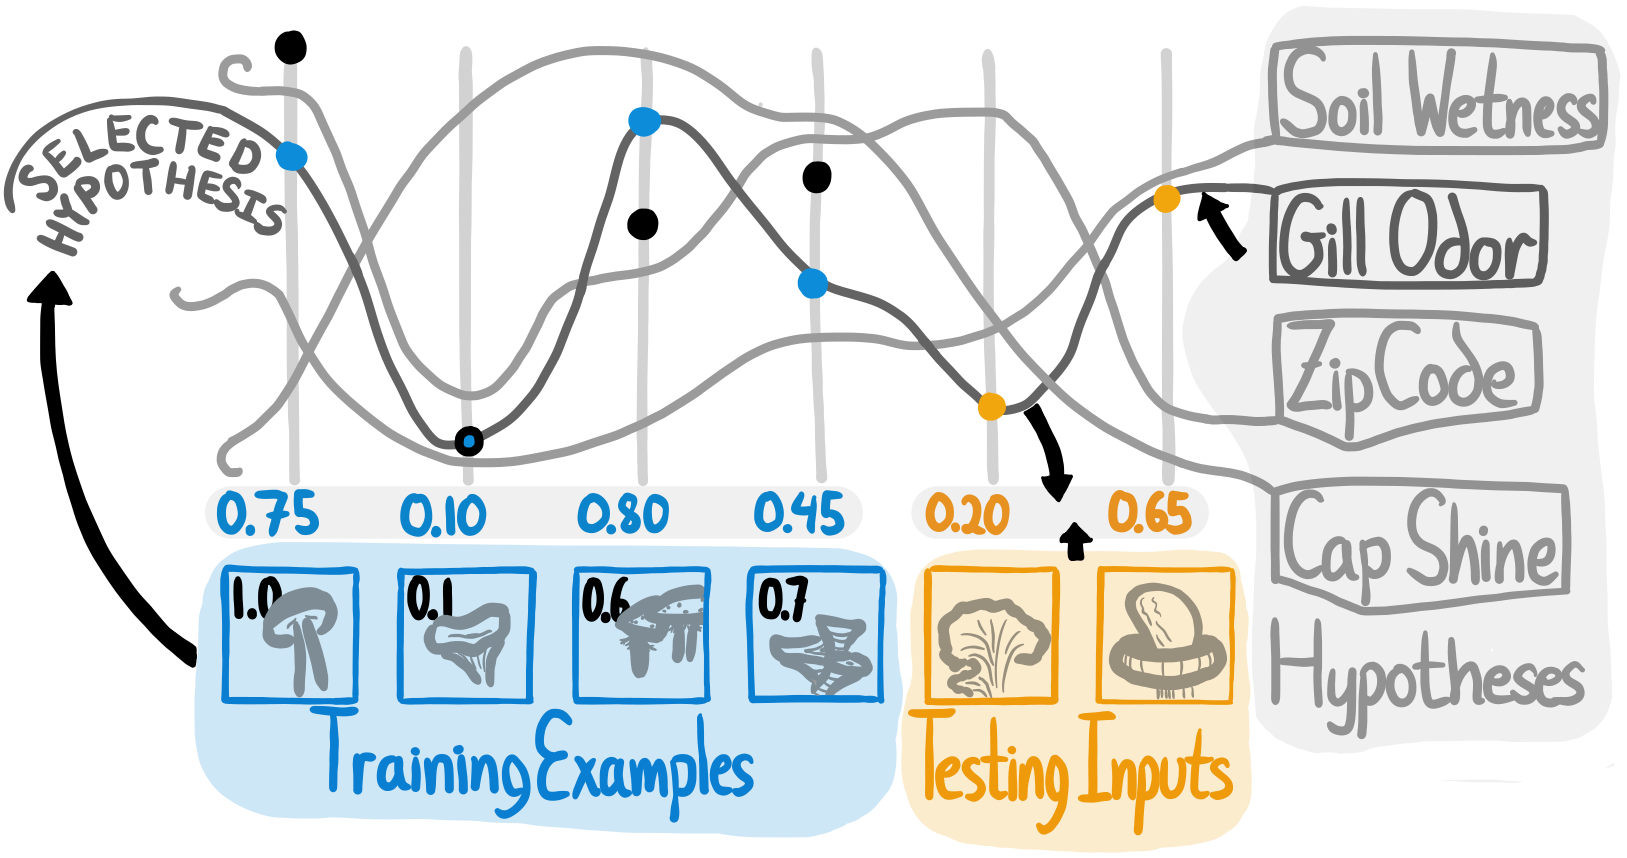
\includegraphics[width=\textwidth]{figures/ml-dataflow}
    \caption{%
      \textbf{Predicting mushrooms' poisons.}
      %
      Our learning program selects from a class of hypotheses ({\gre gray blob}) a plausible
      hypothesis that well fits (\textbf{\blu blue dots} are close to
      \textbf{black dots}) a given list of poison-labeled mushrooms ({\blu blue
      blob}).  Evaluating the selected hypothesis on new mushrooms, we predict
      the corresponding poison levels ({\rng orange numbers}).
      %
      \par The arrows show dataflow: how the hypothesis class and the
      mushroom+poisonlevel examples determine one hypothesis, which, together
      with new mushrooms, determines predicted poison levels.
      %
      Selecting a
      hypothesis is called \textbf{learning}; predicting unseen poison levels,
      \textbf{inference}.  The examples we learn from are
      \textbf{training data}; the new mushrooms and their true poison levels
      are \textbf{testing data}.
    }
    \vspace{-1.0cm}
  \end{figure}

  For example, say we want to predict poison levels (answers) of mushrooms
  (prompts).  %Comparing our `\textbf{training data}' to our
  Among our hypotheses,\bovinenote{%
      We choose four hypotheses: respectively, that
      a mushroom's poison level is
      close to:
      \par\emph{--- its ambient soil's percent water by weight};
      \par\emph{--- its gills' odor level, in kilo-Scoville units};
      \par\emph{--- its zipcode (divided by 100000)};
      \par\emph{--- the fraction of visible light its cap reflects}.
  }
  the GillOdor hypothesis fits the examples well: it guesses poison
  levels
  %(\textbf{\blu blue dots})
  close to the truth.
  %(\textbf{black dots}).
  So the program selects GillOdor.
 %(jargon: \textbf{learns})
  %The selection process is called \textbf{learning}.

  `\emph{Wait!}', you say,
  `\emph{doesn't Zipcode fit the example data more closely than GillOdor?'}.
  Yes.  But a poison-zipcode proportionality is implausible: we'd need
  more evidence before believing Zipcode.  We can easily make many oddball
  hypotheses; by chance some may fit our data well, but they probably
  won't predict well!
  %
  Thus
  ``intrinsic plausibility'' and ``goodness-of-fit-to-data''
  \emph{both}\bovinenote{%
    We choose those two notions (and our $\hH$) based on \textbf{domain
    knowledge}.  This design process is an art; we'll study some rules of
    thumb.
  } play a role in learning.

  %We must specify both notions based on our domain knowledge
  %--- this is an art but we'll learn its rules of thumb.
  %
  %We've now met ML's key elements.
  %Those are ML's elements.
  In practice we'll think of each hypothesis as mapping mushrooms to
  \emph{distributions} over poison levels; then its
  ``goodness-of-fit-to-data'' is simply the chance it allots to the
  data.\bovinenote{That's why we'll need \textbf{probability}.}
  %the details are more complex.
  We'll also use huge $\hH$s: we'll \emph{combine} mushroom features
  (wetness, odor, and shine) to make more hypotheses such as
  %Maybe
  $
    (1.0 \cdot \text{GillOdor} - 0.2\cdot \text{CapShine})
  $.\bovinenote{That's why we'll need \textbf{linear algebra}.}
  %predicts poison well!
  %
  Since we can't compute ``goodness-of-fit'' for so many hypotheses,
  we'll guess a hypothesis
  %start at a tentative hypothesis and
  then repeatedly
  nudge it up the ``goodness-of-fit'' \emph{slope}.\bovinenote{That's why we'll need \textbf{derivatives}.}
  %
  %

  %We must specify both notions based on our domain knowledge
  %--- this is an art but we'll learn its rules of thumb.
  %%
  %We'll often do this in terms of \emph{probabilities}:\bovinenote{%
  %  Still, probability isn't the only criterion: if overestimating poison
  %  levels is safer than underestimating them, then we'd want to hedge toward
  %  overestimating.
  %  This will become especially unavoidable when in Unit 5 we learn
  %  from reinforcement.
  %}
  %we supply a distribution over all hypotheses (a \textbf{prior}) and, we think
  %of each hypothesis as mapping mushrooms to \emph{distributions} over poison
  %levels.

  %\bovinenote{%
  %    \textbf{Bayesian Information Criterion}
  %}

\sampassage{supervised learning}
  We'll soon allow uncertainty by letting patterns map prompts to
  \emph{distributions} over answers.
  %\bovinenote{%
  %  Then learning programs have this type:
  %  $$
  %    \lL : (\xX\times \yY)^N \to (\xX\to \text{DistributionsOn}(\yY))
  %  $$
  %}
  %
  Even if there is only one prompt --- say, ``\emph{produce a
  beautiful melody}'' --- we may seek to learn the complicated
  distribution over answers, e.g.\ to generate a diversity of apt
  answers.  Such \textbf{unsupervised learning} concerns output
  structure.
  %
  By contrast, \textbf{supervised learning} (our main subject), concerns
  the input-output relation; it's interesting when there are many possible prompts.
  %there are many possible prompts.
  %
  Both involve learning from examples; the distinction is no more firm
  than that between sandwiches and hotdogs, but the words are good to
  know.

  %To save ink, say that $\xX$ is the set of possible prompts; $\yY$, of
  %possible answers.
  %%
  %With the example above, $\xX$ contains all
  %conceivable mushrooms and $\yY$ contains all conceivable poison
  %levels (perhaps all the non-negative real numbers).
  %%
  %If we like, we can now summarize the data flow in symbols.  A pattern is a
  %function of type $\xX\to\yY$.  And we can model the examples from which our
  %program learns as a list of type $(\xX\times \yY)^N$.  Then a program that
  %learns from examples has type:
  %$$
  %  \lL : (\xX\times \yY)^N \to (\xX\to \yY)
  %$$

%\sampassage{learning as...}
%  TODO
%    %
%\attnsam{
%    machine learning is like science.
%    %
%    machine learning is like automatic programming.
%    %
%    machine learning is like curve-fitting.
%    %%
%    three classic threads of AI
%    }

    \samsection{our first learning algorithm}
      \hypertarget{A2}{}
      \objectives{%
    \item write a simple, inefficient image classifier %ying ML program
    \item visualize data as lying in feature space; visualize hypotheses as
            functions defined on feature space; and visualize the class of
            all hypotheses within weight space
}

%%\samsection{a tiny example: handwritten digit classification}
%      \samquote{
%        The learning process is something you can incite, literally incite, like a riot.
%      }{audre lorde}

%~~~~~~~~~~~~~~~~~~~~~~~~~~~~~~~~~~~~~~~~~~~~~~~~~~~~~~~~~~~~~~~~~~~~~~~~~~~~~~
%~~~~~~~~~~~~~  1.3. meeting the data  ~~~~~~~~~~~~~~~~~~~~~~~~~~~~~~~~~~~~~~~~

\sampassage{meeting the data}
  Say we want to classify handwritten digits.
  In symbols: we'll map $\xX$ to $\yY$ with $\xX =
  \{\text{grayscale~}28\!\times\!28\text{-pixel images}\}$,
  $\yY=\{{\blu{1}},{\rng{3}}\}$.
  Each datum $(x,y)$ arises as follows: we randomly choose a digit $y\in \yY$,
  ask a human to write that digit in pen, and then photograph their writing to
  produce $x\in\xX$.
  %
  \newcommand{\mnistex}[2]{%
      \includegraphics[width=0.75cm]{example-mnist/mnist-trn-#1}\vspace{-0.2cm}%
      \\#2%
  }
  \vspace{-0.25cm}
  \begin{figure}
      \centering
    \vspace{+0.15cm}%
    \begin{tabular}{c}\mnistex{00}{$\rng{3}$}\\\mnistex{10}{$\rng{3}$}\end{tabular}%
    \begin{tabular}{c}\mnistex{01}{$\blu{1}$}\\\mnistex{11}{$\blu{1}$}\end{tabular}%
    \begin{tabular}{c}\mnistex{02}{$\rng{3}$}\\\mnistex{12}{$\rng{3}$}\end{tabular}%
    \begin{tabular}{c}\mnistex{03}{$\rng{3}$}\\\mnistex{13}{$\blu{1}$}\end{tabular}%
    \begin{tabular}{c}\mnistex{04}{$\rng{3}$}\\\mnistex{14}{$\rng{3}$}\end{tabular}%
    \begin{tabular}{c}\mnistex{05}{$\blu{1}$}\\\mnistex{15}{$\blu{1}$}\end{tabular}%
    \begin{tabular}{c}\mnistex{06}{$\blu{1}$}\\\mnistex{16}{$\rng{3}$}\end{tabular}%
    \begin{tabular}{c}\mnistex{07}{$\rng{3}$}\\\mnistex{17}{$\blu{1}$}\end{tabular}%
    \begin{tabular}{c}\mnistex{08}{$\rng{3}$}\\\mnistex{18}{$\rng{3}$}\end{tabular}%
    \begin{tabular}{c}\mnistex{09}{$\rng{3}$}\\\mnistex{19}{$\blu{1}$}\end{tabular}%
    \caption{%
      Twenty example pairs.  Each photo $x$ is a $28\times 28$ grid of
      numbers representing pixel intensities.  The light gray background
      has intensity $0.0$; the blackest pixels, intensity $1.0$.  Below
      each photo $x$ we display the corresponding label $y$:
      either $y= {\blu{1}}$ or
      $y={\rng{3}}$.
      %
      We'll adhere to this color code throughout this tiny example.
    }
  \end{figure}

  \begin{marginfigure}[2.5cm]
    \center
    
\includegraphics[width=0.45\textwidth]{example-mnist/mnist-trn-01}%
    \hspace{0.5cm}%
    
\includegraphics[width=0.45\textwidth]{example-mnist/mnist-trn-00}%
  \end{marginfigure}
  When we zoom in, we can see each photo's $28\times 28$ grid of pixels.
  On the computer, this data is stored as a $28\times 28$ grid of
  numbers: $0.0$ for bright through $1.0$ for dark.  We'll name these
  $28\times28$ grid locations by their row number (counting from
  the top) followed by their column number (counting from the
  left).  So location $(0,0)$ is the upper left corner pixel;
  $(27,0)$, the lower left corner pixel.
  \par\noindent
  \exercise{Where is location $(0,27)$?  %$(14,8)$?
  Which way is $(14,14)$ off-center?}

  To get to know the data, let's wonder how we'd hand-code a
  classifier (worry not: soon we'll do this more automatically).
  We want to complete the code
  %
  \begin{lstlisting}[language=Python, basicstyle=\footnotesize\ttfamily]
    def hand_coded_predict(x):
      return 3 if condition(x) else 1
  \end{lstlisting}
  %
  Well, ${\rng{3}}$s tend to have more ink than than ${\blu{1}}$s ---
  should \texttt{condition}\ threshold by the photo's brightness?
  %
  Or: ${\blu{1}}$s and ${\rng{3}}$s tend to have different widths ---
  should \texttt{condition}\ threshold by the photo's dark part's width?

  To make this precise, let's define a photo's \emph{brightness} as $1.0$ minus
  its average pixel darkness; its \emph{width} as the standard deviation of
  the column index of its dark pixels.
    Such
  functions from inputs in $\xX$ to numbers are called
  \textbf{features}.
      %return np.mean(np.mean(x, axis=0), axis=0)
  \begin{lstlisting}[language=Python, basicstyle=\footnotesize\ttfamily]
    SIDE = 28
    def brightness(x):  return 1. - np.mean(x)
    def width(x):       return np.std([col for col in range(SIDE)
                                           for row in range(SIDE)
                                           if 0.5 < x[row][col]  ])/(SIDE/2.0)
    # (we normalized width by SIDE/2.0 so that it lies within [0., 1.]) 
  \end{lstlisting}
  %\par\noindent
  %\begin{figure}[h]
  \begin{marginfigure}[-2.5cm]
    \centering
    %\vspace{-3.5cm}
    %
\includegraphics[width=0.24\textwidth]{example-mnist/mnist-trn-00}
    %
\includegraphics[width=0.24\textwidth]{example-mnist/mnist-trn-01}
    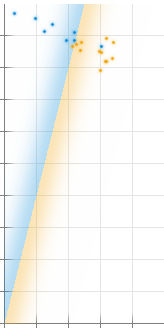
\includegraphics[width=0.85\textwidth]{example-mnist/train-plain-cropped}
    \caption{%
      \textbf{Featurized training data.}
      Our $N=20$ many training examples, viewed in the
      brightness-width plane.  The vertical \emph{brightness} axis ranges
      $[0.0,1.0]$; the horizontal \emph{width} axis ranges $[0.0,0.5]$.
      The origin is at the lower left.  {\rng{Orange}} dots represent
      $y={\rng{3}}$ examples; {\blu{blue}} dot, $y={\blu{1}}$ examples.
      %
      We eyeballed the line $-1\cdot \text{brightness} +4\cdot\text{width}=0$
      to separate the two kinds of examples.
      %
      %The big ${\rng{3}}$ above has brightness and width $(0.118, 0.375)$;\
      %the big ${\blu{1}}$, $(0.092, 0.404)$.  See where they are in this
      %plot?
    }
  \end{marginfigure}
  %\end{figure}

  So we can threshold by brightness or by width.  But this isn't very
  satisfying, since sometimes there are especially dark ${\blu{1}}$s or
  thin ${\rng{3}}$s.
  %
  Aha!  Let's use \emph{both} features: ${\rng{3}}$s are darker than
  ${\blu{1}}$s \emph{even relative to their width}.  Inspecting the
  training data, we see that a line through the origin of slope $4$
  roughly separates the two classes.  So let's
  threshold by a combination like \texttt{-1*brightness(x)+4*width(x)}:
  %\bovinenote{%
  %  \blarr That factor of $2$ comes from our observation that brightness
  %  tends to be bigger than width.  We'll soon see that this eyeballed
  %  slope doesn't work well.  It's better to tune by machine.
  %}
  \begin{lstlisting}[language=Python, basicstyle=\footnotesize\ttfamily]
    def condition(x):
      return -1*brightness(x)+4*width(x) > 0
  \end{lstlisting}
  Intuitively, the formula $-1\cdot \text{brightness} +4\cdot\text{width}$ we
  invented is a measure of \emph{threeness}: if it's positive, we predict
  $y={\rng 3}$.  Otherwise, we predict $y={\blu 1}$.
  %\exercise{Guess a good pair $(a,b)$ based on the training data.}
  %\exercise{Implement a crude ``hole-detector'' feature.  False positives are
  %okay.}
  %\exercise{Make a width feature.  Plot the training data in the
  %width-width plane.}
  \exercise{%
      What further features might help us separate digits
        ${\blu{1}}$ from ${\rng{3}}$?
  }



\pagebreak
\sampassage{candidate patterns}
  We can generalize the hand-coded hypothesis from the previous passage
  to other coefficients besides $-1\cdot \text{brightness}(x) +4\cdot\text{width}(x)$.  We let our set $\hH$ of candidate patterns
  contain all ``linear hypotheses'' $f_{a,b}$ defined by:
  $$
    f_{a,b}(x) = {\rng{3}} \text{~~if~~} a\cdot\text{brightness}(x) + b\cdot\text{width}(x) > 0 \text{~~else~~} {\blu{1}}
  $$
  Each $f_{a,b}$ makes predictions of $y$s given $x$s.  As we change $a$
  and $b$, we get different predictors, some more accurate than others.
  \begin{marginfigure}[-0.0cm]
      \centering
      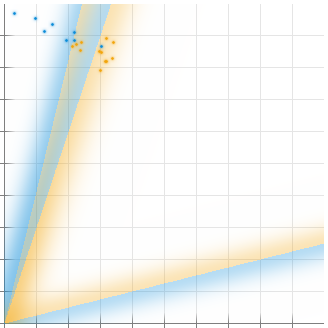
\includegraphics[width=0.99\textwidth]{example-mnist/train-features.png}%
      %
      \caption{%
        \textbf{Hypotheses differ in training accuracy: feature space.}
        %
        $3$ hypotheses classify training data in the brightness-width
        plane (axes range $[0, 1.0]$).
        Glowing colors distinguish a
        hypothesis' $\blu{1}$ and $\rng{3}$ sides.
        For instance, the bottom-most line classifies all the training points
        as $\rng{3}$s.
        %
        \textbf{Caution}: the colors in this page's two Figures
        represent unrelated distinctions!
      }
      \label{fig:train-features}
  \end{marginfigure}

  \begin{lstlisting}[language=Python, basicstyle=\footnotesize\ttfamily]
    def predict(x,a,b):
      return 3 if a*brightness(x) + b*width(x) > 0 else 1
  \end{lstlisting}
  The brightness-width plane is called \textbf{feature space}: its points
  represent inputs $x$ in terms of chosen features (here, brightness and
  width).  The $(a,b)$ plane is called \textbf{weight space}: its points
  represent linear hypotheses $h$ in terms of the coefficients --- or \textbf{weights} ---
  $h$ places on each feature (e.g. $a=-1$ on brightness and $b=+4$ on width).

  \exercise{Which of Fig.\ \ref{fig:train-features}'s $3$ hypotheses best predicts training data?
  }

  \exercise{What $(a,b)$ pairs might have produced Fig.\
  \ref{fig:train-features}'s $3$ hypotheses?  Can you determine $(a,b)$
  for sure, or is there ambiguity (i.e., can multiple $(a,b)$ pairs make
  exactly the same predictions in brightness-width space)?
  }

%~~~~~~~~~~~~~~~~~~~~~~~~~~~~~~~~~~~~~~~~~~~~~~~~~~~~~~~~~~~~~~~~~~~~~~~~~~~~~~
%~~~~~~~~~~~~~  1.5. optimization  ~~~~~~~~~~~~~~~~~~~~~~~~~~~~~~~~~~~~~~~~~~~~

\sampassage{optimization}
  Let's write a program to automatically find hypothesis $h=(a,b)$ from the
  training data.  We want to predict the labels $y$ of yet-unseen photos $x$
  (\emph{testing examples}); insofar as training data is representative of
  testing data, it's sensible to return a $h\in \hH$ that correctly classifies
  maximally many training examples.

  %%Let's write a program $\lL$ that given a list of \emph{training
  %%examples} produces a hypothesis in $h \in \hH$ that helps us predict
  %%the labels $y$ of yet-unseen photos $x$ (\emph{testing examples}).
  %%Insofar as training data is representative of testing data, it's
  %%sensible to return a $h\in \hH$ that correctly classifies maximally
  %%many training examples.
  %
  To do this, let's just loop over a bunch $(a,b)$s --- say, all integer
  pairs in $[-99,+99]$ --- and pick one that misclassifies the least
  training examples:
  \begin{lstlisting}[language=Python, basicstyle=\footnotesize\ttfamily]
    def is_correct(x,y,a,b):
      return 1.0 if predict(x,a,b)==y else 0.0
    def accuracy_on(examples,a,b):
      return np.mean(is_correct(x,y,a,b) for x,y in examples)
    def best_hypothesis():
      # returns a pair (accuracy, hypothesis)
      return max((accuracy_on(training_data, a, b), (a,b))
                 for a in np.arange(-99,+100)
                 for b in np.arange(-99,+100)             )
  \end{lstlisting}

  %%\begin{figure}[h]
  \begin{marginfigure}[-2.2cm]
      \centering
      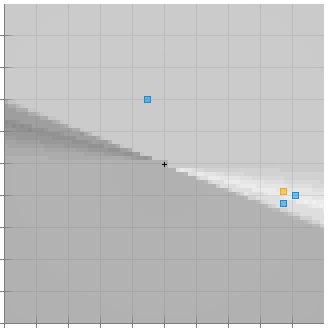
\includegraphics[width=0.99\textwidth]{example-mnist/train-weights.png}\\%
      %
      \caption{%
        \textbf{Hypotheses differ in training accuracy: weight space.}
        %
        We visualize $\hH$ as the $(a,b)$-plane (axes range
        $[-99,+99]$).  Each point determines a whole line in the
        brightness-width plane.  Shading shows training error: darker points
        misclassify more training examples.  The least shaded, most training-accurate
        hypothesis is $(-20, 83)$: the rightmost of the $3$
        {\blu blue squares}.
        %
        The {\rng orange square} is the hypothesis that best fits our unseen
        testing data.
        %--- in the real world we can't compute it but in this toy
        %example we can.
        %
        %
        %\par\noindent
    \exercise{Suppose Fig.\ \ref{fig:train-features}'s $3$ hypotheses arose
    from Fig.\ \ref{fig:train-weights}'s $3$ {\blu blue squares}.
    Which hypothesis matches each square?}
      }
      \label{fig:train-weights}
  \end{marginfigure}



%(0, -2.0, 8.25) reduces train error to 0.10; has test error 0.17
%(0, -1.75, 7.5) reduces test error to 0.15; has train error 0.15

  Fed our $N=20$ training examples, the loop finds
  $(a,b)=(-20,+83)$ as a minimizer of \textbf{training error}, i.e.,
  of the fraction of training examples misclassified.  It misclassifies
  only $10\%$ of training examples. Yet the same
  hypothesis misclassifies a greater fraction --- $17\%$ --- of fresh,
  yet-unseen testing examples.
  %
  That latter number --- called the \textbf{testing error} --- represents
  our program's accuracy ``in the wild''; it's the number we most care
  about.

  The difference between training and testing error is the
  difference between our score on our second try on a practice exam (after we've reviewed
  our mistakes) versus our score on a real
  exam (where we don't know the questions beforehand and aren't allowed
  to change our answers once we get our grades back).

      \exercise{In the $(a,b)$ plane shaded by training error, we see two
  `cones', one dark and one light.  They lie geometrically opposite to each
      other --- why?}

  \exercise{Sketch $f_{a,b}$'s error on $N=1$ example as a
  function of $(a,b)$.}


%    
\includegraphics[width=0.75cm]{example-mnist/mnist-trn-10}\vspace{-0.2cm}\\$\blu{1}$\end{tabular}%
%    \begin{tabular}{c}
\includegraphics[width=0.75cm]{example-mnist/mnist-trn-01}\vspace{-0.2cm}\\$\blu{1}$\\
\includegraphics[width=0.75cm]{example-mnist/mnist-trn-11}\vspace{-0.2cm}\\$\rng{3}$\end{tabular}%
%    \begin{tabular}{c}
\includegraphics[width=0.75cm]{example-mnist/mnist-trn-02}\vspace{-0.2cm}\\$\rng{3}$\\
\includegraphics[width=0.75cm]{example-mnist/mnist-trn-12}\vspace{-0.2cm}\\$\blu{1}$\end{tabular}%
%    \begin{tabular}{c}
\includegraphics[width=0.75cm]{example-mnist/mnist-trn-03}\vspace{-0.2cm}\\$\rng{3}$\\
\includegraphics[width=0.75cm]{example-mnist/mnist-trn-13}\vspace{-0.2cm}\\$\blu{1}$\end{tabular}%
%    \begin{tabular}{c}
\includegraphics[width=0.75cm]{example-mnist/mnist-trn-04}\vspace{-0.2cm}\\$\blu{1}$\\
\includegraphics[width=0.75cm]{example-mnist/mnist-trn-14}\vspace{-0.2cm}\\$\rng{3}$\end{tabular}%
%    \begin{tabular}{c}
\includegraphics[width=0.75cm]{example-mnist/mnist-trn-05}\vspace{-0.2cm}\\$\rng{3}$\\
\includegraphics[width=0.75cm]{example-mnist/mnist-trn-15}\vspace{-0.2cm}\\$\rng{3}$\end{tabular}%
%    \begin{tabular}{c}
\includegraphics[width=0.75cm]{example-mnist/mnist-trn-06}\vspace{-0.2cm}\\$\rng{3}$\\
\includegraphics[width=0.75cm]{example-mnist/mnist-trn-16}\vspace{-0.2cm}\\$\rng{3}$\end{tabular}%
%    \begin{tabular}{c}
\includegraphics[width=0.75cm]{example-mnist/mnist-trn-07}\vspace{-0.2cm}\\$\rng{3}$\\
\includegraphics[width=0.75cm]{example-mnist/mnist-trn-17}\vspace{-0.2cm}\\$\blu{1}$\end{tabular}%
%    \begin{tabular}{c}
\includegraphics[width=0.75cm]{example-mnist/mnist-trn-08}\vspace{-0.2cm}\\$\blu{1}$\\
\includegraphics[width=0.75cm]{example-mnist/mnist-trn-18}\vspace{-0.2cm}\\$\rng{3}$\end{tabular}%
%    \begin{tabular}{c}
\includegraphics[width=0.75cm]{example-mnist/mnist-trn-09}\vspace{-0.2cm}\\$\rng{3}$\\
\includegraphics[width=0.75cm]{example-mnist/mnist-trn-19}\vspace{-0.2cm}\\$\blu{1}$\end{tabular}%
%



    \samsection{how well did we do?  (3 kinds of error : opt, approx, gen)}
      \hypertarget{A2}{}
      \objectives{%
      \item compute and conceptually distinguish training and testing misclassification errors
      \item explain how the problem of achieving low testing error
            decomposes into the three problems of achieving low
            \emph{generalization},
            \emph{optimization}, and
            \emph{approximation}
            errors.
}

\sampassage{error analysis}
  Intuitively, our testing error of $17\%$ comes from three sources:
  \textbf{(a)} the failure of our training set to be representative of our testing set;
  \textbf{(b)} the failure of our program to exactly minimize training error over $\hH$; and
  \textbf{(c)} the failure of our hypothesis set $\hH$ to contain ``the true'' pattern.

  These are respectively errors of
  \textbf{generalization},
  \textbf{optimization},
  \textbf{approximation}.

  We can see generalization error when we plot testing data in the
  brightness-width plane.  The hypotheses $h=(20, 83)$ that we selected based
  on the training in the brightness-width plane misclassifies many testing
  points.  we see many misclassified points.  Whereas $h$ misclassifies only
  $10\%$ of the training data, it misclassifies $17\%$ of the testing data.
  This illustrates generalization error.

  In our plot of the $(a,b)$ plane,
  the {\blu blue square} is the hypothesis $h$ (in $\hH$) that best fits
  the training data.  The {\rng orange square} is the hypothesis (in
  $\hH$) that best fits the testing data.  But even the latter seems
  suboptimal, since $\hH$ only includes lines through the origin while it
  seems we want a line --- or curve --- that hits higher up on the
  brightness axis.  This illustrates approximation error.\bovinenote{%
    To define \emph{approximation error}, we need to specify whether the `truth'
    we want to approximate is the training or the testing
    data.  Either way we get a useful concept.  In this paragraph we're talking
    about approximating \emph{testing} data; but in our notes overall we'll
    focus on the concept of error in approximating \emph{training} data.
  }

  Optimization error is best seen by plotting training rather than testing
  data.  It measures the failure of our selected hypothesis $h$ to minimize
  training error --- i.e., the failure of the {\blu blue square} to lie in a
  least shaded point in the $(a,b)$ plane, when we shade according to training
  error.

  \begin{figure}[h]
  %\begin{marginfigure}%[h]
      \centering
      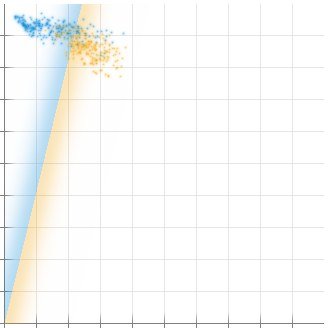
\includegraphics[width=0.49\textwidth]{example-mnist/test-features.png}%
      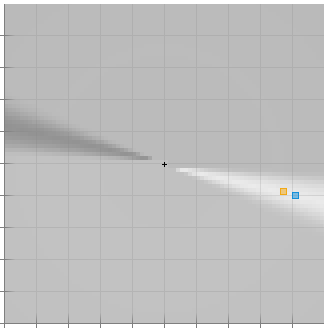
\includegraphics[width=0.49\textwidth]{example-mnist/test-weights.png}%
      %
      \caption{
          \textbf{Testing error visualized two ways.}.
        --- %  \par\noindent
        \textbf{Left: in feature space.}
        The hypotheses $h=(20, 83)$ that we selected based on the training set
        classifies testing data in the brightness-width plane; glowing colors
        distinguish a hypothesis' $\blu{1}$ and $\rng{3}$ sides.
        Axes range $[0, 1.0]$.
        %
        %
        --- %  \par\noindent
        \textbf{Right: in weight space.}
        %
        Each point in the $(a,b)$ plane
        represents a hypothesis; darker regions misclassify a greater
        fraction of testing data.  Axes range $[-99,+99]$.
        %
      }
      \label{fig:test-features-weights}
  \end{figure}
  %\end{marginfigure}

  Here, we got optimization error $\approx 0\%$ (albeit by
  \emph{unscalable brute-force}).  Because optimization error is zero in
  our case, the approximation error and training error are the same:
  $\approx10\%$.  The approximation error is so high because our straight
  lines are \emph{too simple}: brightness and width lose useful
  information and the ``true'' boundary between digits --- even training ---
  may be curved.
  %
  Finally, our testing error $\approx 17\%$ exceeds our training error.
  We thus suffer a generalization error of $\approx 7\%$: we \emph{didn't
  perfectly extrapolate} from training to testing situations.
  %
  In 6.86x we'll address all three italicized issues.

  \exercise{why is generalization error usually positive?}



\sampassage{formalism}\marginnote{\veryoptional}
  Here's how we can describe learning and our error decomposition in
  symbols.
  %
  Draw training examples $\sS : (\xX\times \yY)^N$
  from nature's distribution $\dD$ on $\xX\times \yY$.  A hypothesis
  $f:\xX\to \yY$ has \textbf{training error}
  $
     \Ein(f) = \Pp_{(x,y)\sim \blu{\sS}}[f(x)\neq y]
  $, an average over examples; and \textbf{testing error}
  $
     \Eout(f) = \Pp_{(x,y)\sim \rng{\dD}}[f(x)\neq y]
  $, an average over nature.  A \emph{learning program} is a function
  $
      \lL : (\xX\times \yY)^N \to (\xX\to \yY)
  $; we want to design $\lL$ so that it maps typical $\sS$s to $f$s with
  low $\Eout(f)$.
  %\marginnote{%
  %  %  TODO: mention extereme class-imbalance and bayesian *decision* theory
  %}

  So
  we often define
  $\lL$ to roughly
  minimize $\Ein$ over a
  set $\hH \subseteq (\xX\to \yY)$ of candidate patterns.  Then $\Eout$
  decomposes
  into the failures
  of
  $\Ein$ to estimate $\Eout$ (generalization),
  of
  $\lL$ to minimize $\Ein$ (optimization), and
  of
  $\hH$ to contain
  nature's
  truth (approximation):
  \newcommand{\minf}[1]{{\inf}_{\hH}}
  \begin{align*}
      \Eout(\lL(\sS))
      =~&\Eout(\lL(\sS))      &-\,\,\,&      \Ein(\lL(\sS)) &~\}~~& \text{\textbf{generalization} error} \\
      +~&\Ein(\lL(\sS))       &-\,\,\,& \minf{\hH}(\Ein(f)) &~\}~~& \text{\textbf{optimization} error} \\
      +~&\minf{\hH}(\Ein(f))  &       &                     &~\}~~& \text{\textbf{approximation} error}
  \end{align*}
  These terms are in tension.  For example, as $\hH$ grows, the
  approx.\ error may decrease while the gen.\ error may
  increase --- this is the ``\textbf{bias-variance} tradeoff''.

    \samsection{how can we do better?  (survey of rest of notes)}
      \hypertarget{A2}{}
      
%~~~~~~~~~~~~~~~~~~~~~~~~~~~~~~~~~~~~~~~~~~~~~~~~~~~~~~~~~~~~~~~~~~~~~~~~~~~~~~
%~~~~~~~~~~~~~  1.9. workflow  ~~~~~~~~~~~~~~~~~~~~~~~~~~~~~~~~~~~~~~~~~~~~~~~~

%      \sampassage{workflow}
%      %\sampassage{workflow: framing}
%        We first \emph{frame}: what data will help us solve what problem?  To
%        do this, we \emph{factor} our complex prediction problem into simple
%        classification or regression problems; randomly \emph{split} the
%        resulting example pairs into training, dev(elopment), and testing sets;
%        and \emph{visualize} the training data to weigh our intuitions.
%
%      %\sampassage{workflow: modeling}
%        Next, we \emph{model}: we present the data to the computer so that
%        true patterns are more easily found.
%        %
%        Here we inject our \emph{domain knowledge} --- our human experience and
%        intuition about which factors are likely to help with prediction.
%        %
%        Modeling includes \emph{featurizing} our inputs and choosing
%        appropriate \emph{priors} and \emph{symmetries}.
%
%      %\sampassage{workflow: training}
%        During \emph{training}, the computer searches among candidate patterns
%        for one that explains the examples relatively well.
%        We used brute force above; we'll soon learn faster algorithms
%        such as \emph{gradient descent} on the training set for parameter
%        selection and \emph{random grid search} on the dev set for
%        hyperparameter selection.
%
%      %\sampassage{workflow: harvesting}
%        Finally, we may \emph{harvest}: we derive insights from the pattern
%        itself\bovinenote{%
%            which factors ended up being most important?
%        }
%        and we predict outputs for to fresh inputs.
%        %
%        Qualifying both applications is the pattern's quality.  To assess this,
%        we measure its accuracy on our held-out testing data.




  \sampart{B. auto-predict by fitting lines to examples (unit 1)}
    \phantomsection\label{part:B}
    \samsection{linear approximation}
      \hypertarget{B0}{}
      \objectives{%
  \item define a class of linear, probabilistic hypotheses appropriate
        to a given classification task, by: designing
        features; packaging the coefficients to be learned as a matrix; and
        selecting a probability model (logistic, perceptron, SVM, etc).
  \item compute the loss suffered by a probabilistic hypothesis on given data
}

%-- what it means for "dogness vs catness" to vary linearly (log probabilities as the thing-to-approximate)
%-- linear geometry of feature space
%-- humble models (svm, perceptron, etc)
%-- featurization and readout //  richer outputs : regression and adt structure

\sampassage{two thirds between dog and cow}
  Remember: our Unit 1 motto is to \emph{learn linearities flanked by hand-coded
  nonlinearities}:
  \[
    \xX   \xrightarrow[\text{\color{gray}not learned}]{\text{featurize}}
    \Rr^2 \xrightarrow[\text{\textbf{learned!}}]{\text{linearly combine}}
    \Rr^1 \xrightarrow[\text{\color{gray}not learned}]{\text{read out}}
    \yY
    %\text{DistributionsOn}(\yY)
  \]
  %
  We design the nonlinearities to capture domain knowledge
  about our data and goals.  Here we'll design nonlinearities to help
  model \emph{uncertainty}
  over $\yY$.  We can do this by choosing a different read-out function.  For
  example, representing distributions by objects \texttt{\{3:prob\_of\_three,
  1:prob\_of\_one\}}, we could choose:
  %    prediction = ({9:0.8, 1:0.2} if threeness[0]>0. else {1:0.8, 9:0.2})
  \begin{lstlisting}[language=Python, basicstyle=\footnotesize\ttfamily]
      prediction = {3 : 0.8 if threeness[0]>0. else 0.2,
                    1 : 0.2 if threeness[0]>0. else 0.8 }
  \end{lstlisting}
  If before we'd have predicted ``the label is ${\rng 3}$'', we now
  predict ``the label is ${\rng 3}$ with 80\% chance and ${\blu 1}$ with 20\% chance''.
  This hard-coded 80\% \emph{could} suffice.\bovinenote{%
    As always, it depends on what specific thing we're trying to do!
  }
%{\blu{1}}$ or
%      $y={\rng{9}}
  But
  let's do better: intuitively, a {\rng{3}} is more likely when
  \texttt{threeness} is huge than when \texttt{threeness} is nearly zero.  So
  let's replace that 80\% by some smooth function of
  \texttt{threeness}.  A popular,
  theoretically warranted choice is $\sigma(z) = 1/(1+\exp(-z))$:\bovinenote{%
    $\sigma$, the \textbf{logistic} or \textbf{sigmoid} function, has linear log-odds: $\sigma(z)/(1\!-\!\sigma(z))=\exp(z)/1$.
    %It squashes its input range $(-\infty, +\infty)$ to an output range $(0.,
    %1.)$.
    It tends exponentially to the step function.
    %$0, 1$ as $z \to -\infty, +\infty$.
    It's symmetrical: $\sigma(-z)=1\!-\!\sigma(z)$.  Its derivative
    concentrates near zero: $\sigma\pr(z) = \sigma(z)\sigma(-z)$.
    %It pervades ML.
    \exercise{Plot $\sigma(z)$
    %= 1/(1+\exp(-z))$
    by hand.}
  }
  %  sigma = lambda z : 1./(1.+np.exp(z))
  %  def predict(x):
  \begin{lstlisting}[language=Python, basicstyle=\footnotesize\ttfamily]
      sigma = lambda z : 1./(1.+np.exp(-z))
      prediction = {3 :    sigma(threeness[0]),
                    1 : 1.-sigma(threeness[0]) }
  \end{lstlisting}
  %\bovinenote{%
  %    \attnsam{PICTURE OF CONTOURS! (two angles; different confidences)}
  %}
  Given training inputs $x_i$, a hypothesis will have ``hunches'' about the
  training outputs $y_i$.  Three hypotheses $h_{\text{three!}}$,
  $h_{\text{three}}$, and $h_{\text{one}}$ might, respectively, confidently
  assert $y_{42}={\rng{3}}$; merely lean toward $y_{42}={\rng{3}}$; and think $y_{42}={\blu{1}}$.  If
  in reality $y_{42}={\blu{1}}$ then we'd say $h_{\text{one}}$ did a good job, $h_{\text{three}}$ a bad
  job, and $h_{\text{three!}}$ a very bad job on the $42$nd example.
  %
  So the training set ``surprises'' different hypotheses to different degrees.
  We may seek a hypothesis $h_\star$ that is minimally surprised, i.e., usually
  confidently right and when wrong not confidently so.
  %sense to ask for a hypothesis that maximizes probability.
  In short, by outputting probabilities instead of mere labels, we've earned
  this awesome upshot: \emph{the machine can automatically calibrate its
  confidence levels!}
  %\bovinenote

  %Now, what does this all mean?  \emph{What does it mean for ``dogness vs
  %cowness'' to vary ``linearly''?}

  \attnsam{Confidence on mnist example!}
  \attnsam{(2 pictures, left and right: hypotheses and (a,b plane)}
  %\vspace{8cm}


\sampassage{interpreting weights}
  We note two aspects of the `intuitive logic' of weights.

  Just because two features both correlate with a positive label ($y=+1$)
  doesn't mean both features will have positive weights.  In other words,
  it could be that the \emph{blah}-feature correlates with $y=+1$ in the
  training set and yet, according to the best hypothesis for that
  training set, the bigger a fresh input's blah feature is, the
  \emph{less} likely its label is to be $+1$, all else being equal.  That
  last phrase ``all else being equal'' is crucial, since it refers to our
  choice of coordinates.
  %
  %\attnsam{Illustrate `averaging' of good features vs `correction' of one
  %feature by another (how much a feature correlates with error)}
  %
  %In fact, t This is the difference between \emph{independence} and
  %\emph{conditional independence}.
  See the figure, left
  three panels.

  \begin{marginfigure}[-1cm]
    \centering
    \picturew{0.99\textwidth}{depshear}%
    \caption{%
      \textbf{Relations between feature statistics and optimal weights.}
      Each of these six figures shows a different binary classification task
      along with a maximum-margin hypothesis.  We shade the datapoints that
      achieve the margin.
      %In these examples, \emph{optimal}
      %means ``achieves minimal training error, even if we jiggle the training
      %points a bit''.  That is, we want the dividing line to be as far from
      %the training points as possible, so that small jiggles don't lead to
      %misclassifications.  Intuitively, testing points are jiggled versions of
      %training points, so this seems like a reasonable criterion.  Later we'll
      %see how this arises from theory.
      ---
      \textbf{Left:} \emph{positive weights don't imply positive correlation!}
      ---
      \textbf{Right:}  \emph{presenting the same information in different
      coordinates alters predictions!}
    }
  \end{marginfigure}
  \attnsam{Note on interpreting weights}
  % dependence

  % shearing
  Moreover, transforming coordinates, even linearly, can alter predictions.
  For example, if we shear two features together --- say, by using
  cooktime-plus-preptime and cooktime as features rather than preptime
  and cooktime as features --- this can impact the decision boundary.
  %
  Of course, the decision boundary will look different because we're in
  new coordinates; but we mean something more profound:
    if we train in old coordinates and then predict a datapoint represented in old coordinates,
  we might get a different prediction than
    if we train in new coordinates and then predict a datapoint represented in new coordinates!
  See the figure, right
  three panels: here, the intersection of the two gray lines implicitly marks
  a testing datapoint that experiences such a change of prediction as we adopt
  different coordinates.
  %
  \emph{Intuitively, the more stretched out a feature axis is, the more the
  learned hypothesis will rely on that feature.}
  \exercise{%
    Understand this paragraph from the point of view of the L2 regularizer.
  }

  % stretching
  %Stretching a single feature --- for instance, measuring it in
  %centimeters instead of meters --- can impact the decision boundary
  %as well.  Intuitively, the more stretched out a feature axis is,
  %the more the learned hypothesis will rely on that feature.




\sampassage{designing featurizations}%\marginnote{\veryoptional}% as an art
%\samquote{%
%  He had bought a large map representing the sea,\\
%  Without the least vestige of land:             \\
%  And the crew were much pleased                 \\
%  when they found it to be                       \\
%  A map they could all understand.
%}{charles dodgson}%
  We represent our input $x$ as a fixed-length list of numbers so that we can
  ``do math'' to $x$.  For instance, we could represent a $28\times 28$ photo
  by $2$ numbers: its overall brightness and its dark part's width.  Or we
  could represent it by $784$ numbers, one for the brightness at each of the
  $28\cdot 28=784$ many pixels.  Or by $10$ numbers that respectively measure
  the overlap of $x$'s ink with that of ``representative'' photos of the digits
  $0$ through $9$.

  A way to represent $x$ as a fixed-length list of numbers is a
  \textbf{featurization}.  Each map from raw inputs to numbers is
  a \textbf{feature}.
  %For example, brightness and width are two features.
  %
  %\attnsam{TODO: mention one-hot, etc}
  %\attnsam{TODO: mention LOWRANK (sketching; also, for multiregression)}
  %
  Different featurizations make different
  patterns easier to learn.
  %
  %\marginnote{%
  %    \attnsam{data-based featurizations via kernels}
  %    \attnsam{will soon learn featurizations}
  %    \attnsam{hand featurization in kaggle and medicine}
  %}
  We judge a featurization not in a vacuum but with respect to the kinds of
  patterns we use it to learn. % Good featurizations make task-relevant
  information easy for the machine to use (e.g.\ through apt nonlinearities)
  and throw away task-irrelevant information (e.g. by turning $784$ pixel
  brightnesses to $2$ meaningful numbers).
  %\attnsam{TODO: graphic of separability; and how projection can reduce it}

  Here are two themes in the engineering art of featurization.\bovinenote{%
    For now, we imagine hand-coding our features rather
    than adapting them to training data.
    %
    We'll later discuss adapted features; simple examples
    include thresholding into \textbf{quantiles} based on sorted training data (\emph{Is $x$ more than
    the median training point?}), and choosing
    coordinate transforms that measure similarity to \textbf{landmarks}
    (\emph{How far is $x$ from each of these $5$ ``representative'' training
    points?}).  Deep learning is a fancy example.
  }
  %\begin{description}

  %  \item[\textbf{Predicates}]
  \textbf{Predicates}.
      If domain knowledge suggests some subset
      $S \subseteq \xX$ is salient, then we can define the feature
      $$
        x \mapsto \text{$1$ if $x$ lies in $S$ else $0$}
      $$
      The most important case helps us featurize \emph{categorical} attributes
      (e.g.\ kind-of-chess-piece, biological sex, or letter-of-the-alphabet):
      if an attribute takes $K$ possible values, then each value induces a
      subset of $\xX$ and thus a feature.  These features assemble into a map
      $\xX\to\Rr^K$.  This \textbf{one-hot encoding} is simple, powerful, and
      common.
      %
      Likewise, if some attribute is \emph{ordered} (e.g.\ $\xX$
      contains
          %people and $x<x\pr$ when $x$ descends from $x\pr$.
      geological strata)
      then interesting predicates may include \textbf{thresholds}.
      %
      %\textbf{Binning}.  Conversely, .
      % discrete <--> continuous by softmax, onehot

    %\item[\textbf{Coordinate transforms}]
      %\attnsam{DISTINGUISH BETWEEN TRAINING POINT INDEX vs DIMENSIONS!}
    \textbf{Coordinate transforms}.
      Applying our favorite highschool math functions gives new features
      $
          \tanh(x[0])-x[1],\, |x[1]x[0]| \exp(- x[2]^2),\, \cdots
      $
      from old features $x[0], x[1], \cdots$.
      We choose these functions based on
      domain knowledge; e.g.\ if $x[0], x[1]$ represent two spatial positions,
      then the distance $|x[0]-x[1]|$ may be a useful feature.
      %positions in space, for instance, then we might want
      %    $(x_{20}-x[-])^2 + (x_{21}-x_{1})^2$
      %gives
      %their squared distance.
      %
      One systematic way to include nonlinearities is to include all
      the monomials (such as $x[0] x[1]^2$) with not too many factors ---
      then linear combinations are polynomials
          %so we call this a \textbf{polynomial featurization}.
      %
      The most important nonlinear coordinate transform uses all monomial
      features with $0$ or $1$ many factors --- said plainly, this maps
      $$
        x \mapsto (1, x)
      $$
      This
      is the \textbf{bias trick}.  Intuitively, it allows the machine to learn
      the threshold above which three-ishness implies a three.
  \begin{marginfigure}[-4cm]
    \centering
    \picturew{0.99\textwidth}{bias-trick}%
    \caption{%
        \textbf{The bias trick helps us model `offset' decision boundaries.}
        Here, the origin is the lower right corner closer to the camera.  Our
        raw inputs $x=(x[0],x[1])$ are $2$-dimensional; we can imagine them sitting on the
        bottom face of the plot (bottom ends of the vertical stems).  But,
        within that face, no line through the origin separates the data well.
        By contrast, when we use a featurization $(1,x[0],x[1])$,
        our data lies on the top face of the plot; now
        a plane through the origin (shown) successfully separates the data.
    }
  \end{marginfigure}
  % dependence
  \begin{marginfigure}
    \attnsam{curvy trick}
  \end{marginfigure}



      %increases dimension by one.
      %\textbf{coordinate transforms} --- e.g.\ arctan.
  %\end{description}

  %Caution: a feature $A(\sfx)$ that is statistically independent from
  %$\sfy$ may still be relevant for predicting $\sfy$.\bovinenote{%
  %  Example.  Consider the uniform distribution on the four corners of a
  %  tetrahedron embedded within the corners of a cube \attnsam{TODO:
  %  graphic}.  The three spatial coordinates give three bit-valued random
  %  variables.  Any two of these variables are independent.  But the
  %  three together are dependent.
  %  \attnsam{TODO: also do a decision boundary (simpsons style) graph
  %  illustrating this phenomenon}
  %}
  %For example, if
  %$A, B$ are two features, it is possible that $A(\sfx), \sfy$ are
  %independent and that $B(\sfx), \sfy$ are independent and yet
  %$A(\sfx),B(\sfx), \sfy$ are \emph{dependent}!

  %\attnsam{TODO: example featurization (e.g. MNIST again?)}



  %\par\noindent
  %\attn{Exercise:} {How might our ${\rng{9}}$ vs ${\blu{1}}$ model fail
  %to generalize to photos of unevenly lit paper?  Photos of lined paper?
  %Of chalk on slate?  Of $7$-segment digital displays?
  %\par\noindent
  %\attn{Exercise:} {How might they fail for classifying $3$ vs $8$?}








\sampassage{humble models}
  Let's modify logistic classification to allow for \emph{unknown
  unknowns}. We'll do this by allowing a classifier to allot probability
  mass not only among labels in $\yY$ but also to a special class $\star$
  that means ``no comment'' or ``alien input''.  A logistic classifier
  always sets $p_{\sfy|\sfx}[\star|x] = 0$, but
  %
  other probability models may put nonzero mass on ``no comment''.
  %Different models give different learning programs.
  For example, consider:
  \newcommand{\zp}{\oplus}%u^{\!+\!}}
  \newcommand{\zm}{\ominus}%u^{\!-\!}}
  \begin{table}
    \centering
    \small
    \vspace{-0.3cm}
    \begin{tabular}{RCCCC}
                                  & \textsc{logistic}     & \textsc{perceptron}       & \textsc{svm}              \\\hline %& \textsc{gauss}
        p_{\sfy|\sfx}[+1| x]      & \zp/(\zm+\zp)         &\zp\cdot(\zm\wedge\zp)/2   &\zp\cdot(\zm\wedge\zp/e)/2 \\       %&\zp \cdot \epsilon e^{-d^2/4}
        p_{\sfy|\sfx}[-1| x]      & \zm/(\zm+\zp)         &\zm\cdot(\zm\wedge\zp)/2   &\zm\cdot(\zm/e\wedge\zp)/2 \\       %&\zm \cdot \epsilon e^{-d^2/4}
        p_{\sfy|\sfx}[\star| x]   & 1 - ~\text{above}=0   &1 - ~\text{above}          &1 - ~\text{above}          \\\hline %&1 - ~\text{above}
            %                                                                                                                    %
      \text{outliers}             &\text{responsive}      &\text{robust}              &\text{robust}              \\       %&\text{vulnerable}
      \text{inliers}              &\text{sensitive}       &\text{blind}               &\text{sensitive}           \\       %&\text{blind}
      %\text{humility}             &\text{low}             &\text{low}                 &\text{high-ish}            \\ 
      \text{acc bnd}              &\text{good}            &\text{bad}                 &\text{good}              \\\hline
%                                                                                                                    %
      \text{loss name}            &\text{softplus}(\cdot) &\text{srelu}(\cdot)        &\text{hinge}(\cdot)        \\       %&\text{parab}(\cdot)
      \text{formula}              &\log_2(1+e^{(\cdot)})  &\max(1,\cdot)+1            &\max(1,\cdot+1)            \\       %&(\cdot+1)^2
      \text{update}               &1/(1+e^{+y\frd})          &\text{step}(-y\frd)           &\text{step}(1-y\frd)            %&2(1-yd)
      %\text{humility}             &\text{low}             &\text{medium}              &\text{high}
      % TODO: split outliers/inliers by good or bad (erroneously classified or not?)  so 4 rows instead of 2?
    \end{tabular}
    \caption{%
      \textbf{Three popular models for binary classification.}
      %
      \textbf{Top rows:} Modeled chance given $x$ that $y=+1$, $-1$,
      $\star$.  We use $\frd = \vec w\cdot \vec x$,
      $\oplus=e^{+\frd/2}, \ominus = e^{-\frd/2}$,
      %$u^{\!\pm\!}$ = $e^{\!\pm\! d/2}$,
      $a\wedge b = \min(a,b)$ to save ink.
      %
      \textbf{Middle rows:} All models respond to misclassifications.
      But are they robust
      to well-classified outliers?
      Sensitive to well-classified inliers?
      %
      \textbf{Bottom rows:} For optimization, which we'll
      discuss later, we list (negative log-probability) losses.
      %that arise when maximize likelihood using these models.
      An SGD step looks like
      $$
        \vec w_{t+1} = \vec w_t + \eta \cdot \text{update} \cdot y \vec x
      $$
      %
    }
    \vspace{+0.3cm}
  \end{table}
  \begin{marginfigure}
    \attnsam{graphs of prob}\\
      \vspace{4cm}\\
    \attnsam{graphs of prob}
  \end{marginfigure}

  MLE with the perceptron model or svm model minimizes
  the same thing, but with
  $\text{srelu}(z) = \text{max}(0,z)+1$ or
  $\text{hinge}(z) = \text{max}(0,z+1)$
  instead of $\text{softplus}(z)$.
  %https://www.desmos.com/calculator/3yak0ozell

  Two essential properties of $\text{softplus}$ are that:
  (a) it is convex\bovinenote{%
    A function is \textbf{convex} when its graph is bowl-shaped rather than
    wriggly.  It's easy to minimize convex functions by `rolling downhill',
    since we'll never get stuck in a local wriggle.  Don't worry about
    remembering or understanding this word.
  }
  and
  (b) it upper bounds the step function.
  Note that $\text{srelu}$ and $\text{hinge}$ also enjoy
  these properties.  Property (a) ensures that the optimization problem
  is relatively easy --- under mild conditions, gradient descent will
  find a global minimum.  By property (b), the total loss
  on a training set upper bounds the rate of erroneous classification on
  that training set.  So loss is a \emph{surrogate} for (in)accuracy: if
  the minimized loss is nearly zero, then the training accuracy is nearly
  $100\%$.\bovinenote{%
    The perceptron satisfies (b) in a trivial way that yields a vacuous
    bound of $100\%$ on the error rate.
  }

  So we have a family of related models: \textbf{logistic},
  \textbf{perceptron}, and \textbf{SVM}.  In Project 1 we'll find hypotheses
  optimal with respect to the perceptron and SVM models (the latter under a
  historical name of \textbf{pegasos}), but soon we'll focus mainly on
  logistic models, since they fit best with deep learning.

  %\attnsam{training behavior!!}
  %\attnsam{response to outliers}
  %\attnsam{support vectors}

  \attnsam{DEFINE NOTION OF LOSS!}



%\sampassage{more classes and beyond}
\sampassage{richer outputs: multiple classes}%\marginnote{\veryoptional}%: larger $\yY$
  We've explored hypotheses
  $
    f_{W}(x) = \text{readout}(W \cdot \text{featurize}(x))
  $
  where $W$ represents the linear-combination step we tune to data.
  We began with \textbf{hard binary classification}, wherein we map inputs
  to definite labels (say, $y=\text{cow}$ or $y=\text{dog}$):
  $$
    \text{readout}(\frd) = \text{``$\text{cow}$ if $0\!<\!\frd$ else $\text{dog}$''}
  $$
  We then made this probabilistic using $\sigma$.  In such \textbf{soft binary
  classification} we return (for each given input) a \emph{distribution} over labels:
  $$
    \text{readout}(\frd) =
    \text{``chance $\sigma(\frd)$ of $\text{cow}$;
            chance $1\!-\!\sigma(\frd)$ of $\text{dog}$''}
  $$
  Remembering that $\sigma(\frd) : (1-\sigma(\frd))$ are in the ratio
  $\exp(\frd) : 1$, we rewrite:
  $$
    \text{readout}(\frd) =
    \text{``chance of $\text{cow}$ is $\exp(\frd)/Z_\frd$;
            of $\text{dog}$, $\exp(0)/Z_\frd$''}
  $$

  %Now, I hope you feel bugged by the above formulas' asymmetry --- why
  %should one class count as positive?! --- and does not immediately
  %generalize to multiple classes.

  I hope some of you felt bugged by the above formulas' asymmetry: $W$ measures
  ``cow-ishness minus dog-ishness'' --- why not the other way around?  Let's
  describe the same set of hypotheses but in a more symmetrical way.  A common
  theme in mathematical problem solving is to trade irredundancy for symmetry
  (or vice versa).  So let's posit both
  a $W_{\text{cow}}$ \emph{and}
  a $W_{\text{dog}}$.  One measures ``cow-ishness''; the other,
  ``dog-ishness''.  They assemble to give $W$, which is now a matrix of shape
  $2\!\times\!\text{number-of-features}$.  So $\frd$ is now a list of $2$ numbers:
  $\frd_{\text{cow}}$ and
  $\frd_{\text{dog}}$.
  Now $\frd_{\text{cow}} - \frd_{\text{dog}}$ plays the role that $\frd$
  used to play.

  Then we can do hard classification by:
  $$
    \text{readout}(\frd) = \text{argmax}_{y} \frd_y
  $$
  and soft classification by:
  $$
    \text{readout}(\frd) = \text{``chance of $y$ is $\exp(\frd_y)/Z_\frd$''}
  $$
  To make probabilities add to one, we divide by $Z_\frd = \sum_y
  \exp(\frd_y)$.

  Behold!  By rewriting our soft and hard hypotheses for binary classification,
  we've found formulas that also make sense for more than two classes!  The
  above readout for \textbf{soft multi-class classification} is called
  \textbf{softmax}.
  \begin{marginfigure}
    \attnsam{softmax plot}\\
      \vspace{4cm}\\
    \attnsam{softmax plot}
  \end{marginfigure}



  %For \emph{multi-output soft classification}, we want to report
  %probabilities instead of general real-valued scores.  Probabilities
  %ought to be non-negative and ought to sum to one.  A nice way to turn
  %general numbers to non-negative (in fact, positive) ones is to apply
  %$\exp$.  A nice way to get positive numbers to sum to $1$ is to divide
  %by their sum.  This leads us to \textbf{softmax}:
  %$$
  %  \text{softmax}(\omega_k ~:~ 0\leq k<K) = \left(\frac{\exp(\omega_k)}{\sum_{k^\prime} \exp(\omega_{k^\prime})} ~:~ 0\leq k<K\right)
  %$$

\sampassage{richer outputs: beyond classification}\marginnote[-2.133cm]{\veryoptional}%: larger $\yY$
  By the way, if we're trying to predict a real-valued output instead of a
  binary label --- this is called \textbf{hard one-output regression} --- we can
  simply return $\frd$ itself as our readout:
  $$
    \text{readout}(\frd) = \frd
  $$
  This is far from the only choice!
  For example, if we know that the true
  $y$s will always be positive, then $\text{readout}(\frd) = \exp(\frd)$ may
  make more sense.
    I've encountered a learning task (about alternating current in power lines)
    where what domain knowledge suggested --- and what ended up working best ---
    were trigonometric functions for featurization and readout!
  There are also many ways to return a distribution instead of a number.  One
  way to do such \textbf{soft one-output regression} is to use normal distributions:\bovinenote{%
    Ask on the forum about the world of alternatives and how they
    influence learning!
  }
  $$
    \text{readout}(\frd) = \text{``normal distribution with mean $\frd$ and variance $25$''}
  $$
  Or we could allow for different variances by making $\frd$ two-dimensional
  and saying $\cdots \text{mean $\frd_0$ and variance $\exp(\frd_1)$}$.
  %
  By now we know how to do \textbf{multi-output regression}, soft or hard: just
  %turn $W$ into a matrix of shape
  %$\text{number-of-outputted-numbers}\times\text{number-of-features}$.
  promote $W$ to a matrix with more output dimensions.

  \attnsam{TODO: show pictures of 3 classes, 4 classes (e.g. digits 0,1,8,9)}

  Okay, so now we know how to use our methods to predict discrete labels or
  real numbers.  But what if we want to output structured data like text?  A
  useful principle is to factor the task of generating such ``variable-length''
  data into many smaller, simpler predictions, each potentially depending on
  what's generated so far.  For example, instead of using $W$ to tell us how to
  go from (features of) an image $x$ to a whole string $y$ of characters, we
  can use $W$ to tell us, based on an image $x$ together with a partial string
  $y\pr$, either what the next character is OR that the string should end.  So
  if there are $27$ possible characters (letters and space) then this is a
  $(27+1)$-way classification problem:
  $$
    (\text{Images} \times \text{Strings}) \to
    \Rr^{\cdots} \to
    \Rr^{28} \to
    \text{DistributionsOn}(\{\text{'a'}, \cdots, \text{'z'}, \text{' '}, \text{STOP}\})
  $$
  We could implement this function as some hand-crafted featurization function
  from $\text{Images} \times \text{Strings}$ to fixed-length vectors, followed
  by a learned $W$, followed by softmax.

  %\exercise{
  %  An ``symbolic expression tree'' is something that looks like
  %  \texttt{(((0.686 + x)*4.2)*x)} or
  %  \texttt{((x*5.9) + (x*x + x*(6.036*x)))}.
  %  That is, a tree is either (a tree \texttt{plus} a tree) OR (a tree
  %  \texttt{times} a tree) OR (the symbol \texttt{x}) OR (some real number).
  %  Propose an architecture that, given a short mathematical word problem,
  %  predicts a symbolic expression tree.
  %  Don't worry about featurization.
  %}

  \exercise{%
     A ``phylogenetic tree'' is something that looks like
     $$\texttt{(dog.5mya.(cow.2mya.raccoon))}$$
     or
     $$\texttt{((chicken.63mya.snake).64mya.(cow)).120mya.(snail.1mya.slug)}$$
     That is, a tree is either a pair of trees together with a real number OR a
     species name.  The numbers represent how long ago various clades diverged.
     Propose an architecture that, given a list of species, predicts a
     phylogenetic tree for that species.
     Don't worry about featurization.
  }



        %-- what it means for "dogness vs catness" to vary linearly
        %-- log probabilities as the thing-to-approximate
        %-- humble models (svm, perceptron, etc)
        %-- richer outputs : regression and adt structure
    \samsection{iterative optimization}
      \hypertarget{B1}{}
      \objectives{%
  \item implement gradient descent for any given loss function and (usually)
       thereby automatically and efficiently find nearly-optimal linear
       hypotheses from data
  \item explain why the gradient-update formulas for common linear models are
        sensible, not just formally but also intuitively
}

%\samquote{
%  Hey Jude, don't make it bad \\
%  Take a sad song and make it better \\
%  Remember to let her under your skin \\
%  Then you'll begin to make it \\
%  Better, better, better, better, better, better, ...
%}{paul mccartney, john lennon}

        %-- gradients
        %-- writing out the code : a key exercise ; batches
        %-- setting initialization and learning rate; local minima
        %-- visualizing noise and curvature

\sampassage{(stochastic) gradient descent}
  We seek a hypothesis that is best (among a class $\hH$) according to some
  notion of how well each hypothesis models given data:
  \begin{lstlisting}[language=Python, basicstyle=\footnotesize\ttfamily]
    def badness(h,y,x):
        # return e.g. whether h misclassifies y,x OR h's surprise at seeing y,x OR etc
    def badness_on_dataset(h, examples):
        return np.mean([badness(h,y,x) for y,x in examples])
  \end{lstlisting}
        %#return np.mean([for y,x in examples])

  %For example, out notion of goodness might map $h$ to its
  %training accuracy $1-\Ein$.  Or, when $h$ has a probabilistic interpretation,
  %our notion of goodness might map $h$ to the probability it predicts for the
  %training outputs $y_i$.\bovinenote{%
  %  In either case, we view our notion-of-good, computed on the training data,
  %  as an estimate of the notion-of-good we most care about: testing
  %  performance.  So $1-\Ein$ estimates $1-\Eout$ and $p(y_i|x_i;h)$ for $y_i,
  %  x_i$ a training example estimates $p(y|x;h)$ for $y,x$ fresh data.
  %}
  %
  Earlier we found a nearly best candidate by brute-force search over all
  hypotheses.  But this doesn't scale to most interesting cases wherein $\hH$
  is intractably large.
  %
  So: \emph{what's a faster algorithm to find a nearly best candidate?}

  A common idea is to start arbitrarily with some $h_0\in \hH$ and
  repeatedly improve to get $h_1, h_2, \cdots$.  We eventually stop, say at $h_{10000}$.
  The key question is:\bovinenote{%
    Also important are the questions of where to start and when to stop.
    But have patience!  We'll discuss these later.
  }
  \emph{how do we compute an improved hypothesis $h_{t+1}$ from our current
  hypothesis $h_t$}?

  We \emph{could} just keep randomly nudging $h_t$ until we hit on an
  improvement; then we define $h_{t+1}$ as that improvement.  Though this
  sometimes works surprisingly well,\bovinenote{%
    If you're curious, search `metropolis hastings' and
    `probabilistic programming'.
  } we can often save time by exploiting more available information.
  Specifically, we can inspect $h_t$'s inadequacies to inform our proposal
  $h_{t+1}$.
  %
  Intuitively, if $h_t$ misclassifies a particular $(x_i, y_i) \in \sS$, then
  we'd like $h_{t+1}$ to be like $h_t$ but nudged toward
  accurately classifying $(x_i, y_i)$.\bovinenote{%
    In doing better on the $i$th datapoint, we might mess up how we do
    on the other datapoints!  We'll consider this in due time.
  }

  How do we compute ``{a nudge toward accurately classifying $(x, y)$}''?  That
  is, how do measure how slightly changing a parameter affects some result?
  Answer: derivatives!  To make $h$ less bad on an example $(y, x)$, we'll
  nudge $h$ in tiny bit along $-g = -d \texttt{badness}(h,y,x) /
  dh$. Say, $h$ becomes $h-0.01g$.\bovinenote{%
    E.g.\ if each $h$ is a vector and we've chosen
    $\texttt{badness}(h,y,x) = -y h\cdot x$ as our notion of badness, then $-d
    \texttt{badness}(h,y,x) / dh = +yx$, so we'll nudge $h$ in the
    direction of $+yx$.
    \exercise{Is this update familiar?}
  }
  Once we write
  \begin{lstlisting}[language=Python, basicstyle=\footnotesize\ttfamily]
    def gradient_badness(h,y,x):
        # returns the derivative of badness(h,y,x) with respect to h
    def gradient_badness_on_dataset(h, examples):
        return np.mean([gradient_badness(h,y,x) for y,x in examples])
  \end{lstlisting}
  we can repeatedly nudge via \textbf{gradient descent (GD)}, the engine of ML:\bovinenote{%
    \noparexercise{Can GD directly minimize misclassification rate?}
  }
  \begin{lstlisting}[language=Python, basicstyle=\footnotesize\ttfamily]
    h = initialize()
    for t in range(10000):
      h = h - 0.01 * gradient_badness_on_dataset(h, examples)
  \end{lstlisting}
  Since the derivative of total badness depends on all the training data,
  looping $10000$ times is expensive.  So in practice we estimate the needed
  derivative based on some \emph{subset} (jargon: \textbf{batch}) of the
  training data --- a different subset each pass through the loop --- in what's
  called \textbf{stochastic gradient descent (SGD)}:
  \begin{lstlisting}[language=Python, basicstyle=\footnotesize\ttfamily]
    h = initialize()
    for t in range(10000):
      batch = select_subset_of(examples)
      h = h - 0.01 * gradient_badness(h, batch)
  \end{lstlisting}
  \begin{marginfigure}
      \attnsam{cartoon of GD}\\
      \vspace{4cm}\\
      \attnsam{cartoon of GD}
  \end{marginfigure}

  (S)GD requires informative derivatives.  Misclassification rate has
  uninformative derivatives: any tiny change in $h$ won't change the predicted
  labels.  But when we use probabilistic models, small changes in $h$ can lead
  to small changes in the predicted \emph{distribution} over labels.
  %
  To speak poetically: the softness of probabilistic models paves a smooth ramp
  over the intractably black-and-white cliffs of `right' or `wrong'.
  %
  We now apply SGD to maximizing probabilities.

\sampassage{maximum likelihood estimation}
  When we can compute each hypothesis $h$'s asserted probability
  that the training $y$s match the training $x$s, it seems
  reasonable to seek an $h$ for which this probability is maximal.  This
  method is \textbf{maximum likelihood estimation (MLE)}.
  %
  It's convenient for the overall goodness to be a sum (or average) over each
  training example.  But independent chances multiply rather than add:
  rolling snake-eyes has chance $1\!/\!6 \cdot 1\!/\!6$, not $1\!/\!6 + 1\!/\!6$.  So
  we prefer to think about maximizing log-probabilities instead of maximizing
  probabilities --- it's the same in the end.\bovinenote{%
    Throughout this course we make a crucial assumption that our training
    examples are independent from each other.
  }
  By historical
  convention we like to minimize badness rather than maximize goodness, so
  we'll use SGD to \emph{minimize negative-log-probabilities}.
  \begin{lstlisting}[language=Python, basicstyle=\footnotesize\ttfamily]
    def badness(h,y,x):
        return -np.log( probability_model(y,x,h) )
  \end{lstlisting}

  Let's see this in action for the linear logistic model we developed for soft
  binary classification.  A hypothesis $\vec w$ predicts that a (featurized)
  input $\vec x$ has label $y=+1$ or $y=-1$ with chance $\sigma(+ \vec w \cdot \vec x)$
  or $\sigma(- \vec w \cdot \vec x)$:
  $$
    p_{\sfy|\sfx,\sfw}(y|\vec x,\vec w) = \sigma(y \vec w \cdot \vec x)
    \quad\quad
    \text{where}
    \quad\quad
    \sigma(\frd) = 1/(1-\exp(-\frd))
  $$
  So MLE with our logistic model means finding $\vec w$ that \emph{minimizes}
  $$
    -\log\wrap{\text{prob of all $y_i$s given all $\vec x_i$s and $\vec w$}}
    =
    \sum_i -\log(\sigma(y_i \vec w\cdot \vec x_i))
  $$
  The key computation is the derivative of those badness terms:\bovinenote{%
    Remember that $\sigma\pr(z) = \sigma(z)\sigma(-z)$.
    %
    To reduce clutter we'll temporarily write $y \vec w\cdot \vec x$ as $ywx$.
  }
  $$
    \frac{\partial (-\log(\sigma(y w x)))}{\partial w}
    =
    \frac{-\sigma(y w x)\sigma(-y w x) y x}{\sigma(y w x)}
    =
    - \sigma(-y w x) y x
  $$

  \exercise{If you're like me, you might've zoned out by now.  But this stuff
  is important, especially for deep learning!  So please graph the
  above expressions to convince yourself that our formula for derivative
  makes sense visually.}

  \vspace{\baselineskip}

  To summarize, we've found the loss gradient for the logistic model:
  \begin{lstlisting}[language=Python, basicstyle=\footnotesize\ttfamily]
    sigma = lambda z : 1./(1+np.exp(-z))
    def badness(w,y,x):             return -np.log( sigma(y*w.dot(x)) )
    def gradient_badness(w,y,x):    return -sigma(-y*w.dot(x)) * y*x
  \end{lstlisting}
  As before, we define overall badness on a dataset as an average badness over
  examples; and for simplicity, let's intialize gradient descent at $h_0=0$:
  \begin{lstlisting}[language=Python, basicstyle=\footnotesize\ttfamily]
    def gradient_badness_on_dataset(h, examples):
      return np.mean([gradient_badness(h,y,x) for y,x in examples])
    def initialize():
        return np.zeros(NUMBER_OF_DIMENSIONS, dtype=np.float32)
  \end{lstlisting}
  Then we can finally write gradient descent:
  \begin{lstlisting}[language=Python, basicstyle=\footnotesize\ttfamily]
    h = initialize()
    for t in range(10000):
      h = h - 0.01 * gradient_badness_on_data(h, examples)
  \end{lstlisting}

  %\attnsam{mention convexity and convergence?}

  \begin{marginfigure}
     \attnsam{show trajectory in weight space over time -- see how certainty
  degree of freedom is no longer redundant? (``markov'')}\\
      \vspace{4cm}\\
    \attnsam{show training and testing loss and acc over time}
  \end{marginfigure}



  \newpage
\sampassage{initialization, learning rate, local minima}\marginnote{\veryoptional}

\sampassage{pictures of training: noise and curvature}\marginnote{\veryoptional}
  \par\attnsam{}
  \par\attnsam{}
  \par\attnsam{test vs train curves: overfitting}
  \par\attnsam{random featurization: double descent}

\sampassage{practical implementation: vectorization}


%    \samsection{5. ideas in optimization}
%      \samquote{
%        premature optimization is the root of all evil
%      }{donald knuth}
%
%        \attn{learning rate as metric; robustness to 2 noise structures}
%        \attn{nesterov momentum}
%        \attn{decaying step size; termination conditions}
%        \attn{batch normalization}
%
%
%
%%~~~~~~~~~~~~~~~~~~~~~~~~~~~~~~~~~~~~~~~~~~~~~~~~~~~~~~~~~~~~~~~~~~~~~~~~~~~~~~
%%~~~~~~~~~~~~~  2.20. local minima  ~~~~~~~~~~~~~~~~~~~~~~~~~~~~~~~~~~~~~~~~~~~
%
%      \sampassage{local minima}
%        % convexity, initialization
%
%%~~~~~~~~~~~~~~~~~~~~~~~~~~~~~~~~~~~~~~~~~~~~~~~~~~~~~~~~~~~~~~~~~~~~~~~~~~~~~~
%%~~~~~~~~~~~~~  2.21. implicit regularization  ~~~~~~~~~~~~~~~~~~~~~~~~~~~~~~~~
%
%      \sampassage{implicit regularization}
%
%%~~~~~~~~~~~~~~~~~~~~~~~~~~~~~~~~~~~~~~~~~~~~~~~~~~~~~~~~~~~~~~~~~~~~~~~~~~~~~~
%%~~~~~~~~~~~~~  2.22. learning rate schedule  ~~~~~~~~~~~~~~~~~~~~~~~~~~~~~~~~~
%
%      \sampassage{learning rate schedule}
%
%%~~~~~~~~~~~~~~~~~~~~~~~~~~~~~~~~~~~~~~~~~~~~~~~~~~~~~~~~~~~~~~~~~~~~~~~~~~~~~~
%%~~~~~~~~~~~~~  2.23. learning rates as dot products  ~~~~~~~~~~~~~~~~~~~~~~~~~
%
%      \sampassage{learning rates as dot products} % connects to whitening / pre-conditioning; ties into next section on kernels
%
%

        %-- gradients
        %-- writing out the code : a key exercise ; batches
        %-- setting initialization and learning rate; local minima
        %-- visualizing noise and curvature
    \samsection{priors and generalization}
      \hypertarget{B2}{}
      %%~~~~~~~~~~~~~~~~~~~~~~~~~~~~~~~~~~~~~~~~~~~~~~~~~~~~~~~~~~~~~~~~~~~~~~~~~~~~~~
%~~~~~~~~~~~~~  2.8. on overfitting  ~~~~~~~~~~~~~~~~~~~~~~~~~~~~~~~~~~~~~~~~~~

      \sampassage{on overfitting}
        In the Bayesian framework, we optimistically assume that our model is
        ``correct'' and that the ``true'' posterior over parameters is
        $$
            p(w|y;x) = p(y|w;x) p(w) / Z_x
        $$
        a normalized product of likelihood and prior.
        %
        Therefore, our optimal guess for a new prediction is:
        $$
            p(y_\star;x_\star, x)
            = \sum_w p(y_\star|w;x_\star) p(y|w;x) p(w) / Z_x
        $$

        For computational tractability, we typically approximate the posterior
        over hypotheses by a point mass at the posterior's mode
        $\text{argmax}_{w^\prime} p(w^\prime|y;x)$:
        $$
            p(w|y,x) \approx \delta(w - w^\star(y,x))
            \quad\quad
            w^\star(y,x)=\text{argmax}_{w^\prime} p(w^\prime|y;x)
        $$
        Then
        $$
            p(y_\star;x_\star, x)
            \approx p(y_\star|w^\star(y,x);x_\star)
        $$

        What do we lose in this approximation?

        \attnsam{$\Ee$ and $\max$ do not commute}

        \attnsam{PICTURE: ``bowtie'' vs ``pipe''}

        \attnsam{BIC for relevant variables}


        %\attnsam{point estimates vs bayesian decision theory}

        %\attnsam{interpolation does not imply overfitting}


%~~~~~~~~~~~~~~~~~~~~~~~~~~~~~~~~~~~~~~~~~~~~~~~~~~~~~~~~~~~~~~~~~~~~~~~~~~~~~~
%~~~~~~~~~~~~~  2.9. log priors and bayes  ~~~~~~~~~~~~~~~~~~~~~~~~~~~~~~~~~~~~

      \sampassage{log priors and bayes}
        \attnsam{fill in computation and bases}
        \attnsam{visual illustration of how choice of L2 dot product matters}
        \attnsam{$\ell^p$ regularization; sparsity}
        \attnsam{eye regularization example!}
        \attnsam{TODO: rank as a prior (for multioutput models)}

        %The so-called $\ell^p$ priors are popular.  For $1\leq p<\infty$,
        %these are defined by:
        For $1\leq p\leq \infty$ and $1\leq q\leq \infty$ we can consider this prior:\bovinenote{%
          To define the cases $p=\infty$ or $q=\infty$ we take limits.
          To define the case $p=\infty=q$ we take limits while maintaining $p=q$.
        }
        $$
            p(w) \propto \exp\left(-\left(\sum_i |\lambda w_i|^p\right)^{q/p}\right)
        $$
        For $q=p$ this decomposes as a sum and thus has each coordinate
        independent.  Whereas $q$ limits outliers, $p$ controls the shape of
        level curves.  Small $q$ makes large vectors more probable and
        small $p$ makes it more probable that the entries within a vector will
        be of very different sizes.
        \newcommand{\priors}[1]{\includegraphics[width=2.9cm]{priors/yo-#1}}
        \newcommand{\smarsh}[1]{\vspace{0.125cm}\smash{\parbox[c]{3cm}{#1}}\vspace{0.525cm}}
        \begin{table}
          \centering
          \begin{tabular}{m{1.1cm}SSS}%
                                & $q=1$                 & $q=2$                 & $q=\infty$              \\%
            \smarsh{     $p=1$} &\smarsh{\priors{1-1}}  &\smarsh{\priors{1-2}}  &\smarsh{\priors{1-inf}}  \\%
            \smarsh{     $p=2$} &\smarsh{\priors{2-1}}  &\smarsh{\priors{2-2}}  &\smarsh{\priors{2-inf}}  \\%
            \smarsh{$p=\infty$} &\smarsh{\priors{inf-1}}&\smarsh{\priors{inf-2}}&\smarsh{\priors{inf-inf}}\\%
          \end{tabular}
        \end{table}

        %\begin{table}
        %    \centering
        %    \begin{tabular}{ccccccc}
        %        p         &       q         &  sample A          &  sample B          &   shape       & indep.?       & outliers    \\\hline% sample A            sample B
        %        $1     $  &       $1$       & $( 0.5,-0.1, 0.7)$ & $(14.4,-0.9,-0.9)$ & octahedron    & $\checkmark$  & many        \\      %$( 0.6, 0.1, 0.9)$  $( 1.6, 0.1, 0.1)$
        %        $1     $  &       $2$       & $( 0.6,-0.1, 0.9)$ & $( 4.8,-0.3,-0.3)$ & octahedron    &               & few         \\      %$( 0.6, 0.1, 0.9)$  $( 1.6, 0.1, 0.1)$
        %        $1     $  &       $\infty$  & $( 0.7,-0.1, 1.1)$ & $( 1.6,-0.1,-0.1)$ & octahedron    &               & none        \\      %$( 0.6, 0.1, 0.9)$  $( 1.6, 0.1, 0.1)$
        %        $2     $  &       $1$       & $( 0.3,-0.2, 0.8)$ & $(13.5,-7.2,-2.7)$ & sphere        &               & many        \\      %$( 0.4, 0.2, 1.0)$  $( 1.5, 0.8, 0.3)$
        %        $2     $  &       $2$       & $( 0.4,-0.2, 1.0)$ & $( 4.5,-2.4,-0.9)$ & sphere        & $\checkmark$  & few         \\      %$( 0.4, 0.2, 1.0)$  $( 1.5, 0.8, 0.3)$
        %        $2     $  &       $\infty$  & $( 0.5,-0.2, 1.2)$ & $( 1.5,-0.8,-0.3)$ & sphere        &               & none        \\      %$( 0.4, 0.2, 1.0)$  $( 1.5, 0.8, 0.3)$
        %        $\infty$  &       $1$       & $( 0.4,-0.2, 0.7)$ & $( 9.0,-8.1,-7.2)$ & cube          &               & many        \\      %$( 0.5, 0.3, 0.9)$  $( 1.0, 0.9, 0.8)$
        %        $\infty$  &       $2$       & $( 0.5,-0.3, 0.9)$ & $( 3.0,-2.7,-2.4)$ & cube          &               & few         \\      %$( 0.5, 0.3, 0.9)$  $( 1.0, 0.9, 0.8)$
        %        $\infty$  &       $\infty$  & $( 0.6,-0.4, 1.1)$ & $( 1.0,-0.9,-0.8)$ & cube          & $\checkmark$  & none        \\      %$( 0.5, 0.3, 0.9)$  $( 1.0, 0.9, 0.8)$
        %    \end{tabular}
        %\end{table}
        %\begin{description}
        %    \item[$(p,q)=(1     ,1)$ --- indep laplacian        ]
        %    \item[$(p,q)=(1     ,2)$ ---                        ]
        %    \item[$(p,q)=(2     ,1)$ ---                        ]
        %    \item[$(p,q)=(2     ,2)$ --- indep\&radial gaussian ]
        %    \item[$(p,q)=(\infty,1)$ ---                        ]
        %    \item[$(p,q)=(\infty,2)$ ---planckian               ]
        %\end{description}

%~~~~~~~~~~~~~~~~~~~~~~~~~~~~~~~~~~~~~~~~~~~~~~~~~~~~~~~~~~~~~~~~~~~~~~~~~~~~~~
%~~~~~~~~~~~~~  2.10. hierarchy, mixtures, transfer  ~~~~~~~~~~~~~~~~~~~~~~~~~~~

      \sampassage{hierarchy, mixtures, transfer}
        \attnsam{k-fold cross validation}
        %\attnsam{dimension-based generalization bound}
        \attnsam{bayesian information criterion}

%~~~~~~~~~~~~~~~~~~~~~~~~~~~~~~~~~~~~~~~~~~~~~~~~~~~~~~~~~~~~~~~~~~~~~~~~~~~~~~
%~~~~~~~~~~~~~  2.11. estimating generalization  ~~~~~~~~~~~~~~~~~~~~~~~~~~~~~~

      \sampassage{estimating generalization}
        \attnsam{k-fold cross validation}
        \attnsam{dimension-based generalization bound}
        \attnsam{bayesian information criterion}

      \newpage
    \samsection{3. model selection}
      \samquote{
        All human beings have three lives: public, private, and secret.
      }{gabriel garc\`ia marquez}



      \objectives{%
  \item implement gradient descent for any given loss function and (usually)
       thereby automatically and efficiently find nearly-optimal linear
       hypotheses from data
}

%\samquote{
%  Hey Jude, don't make it bad \\
%  Take a sad song and make it better \\
%  Remember to let her under your skin \\
%  Then you'll begin to make it \\
%  Better, better, better, better, better, better, ...
%}{paul mccartney, john lennon}

        %-- gradients
        %-- writing out the code : a key exercise ; batches
        %-- setting initialization and learning rate; local minima
        %-- visualizing noise and curvature

\sampassage{(stochastic) gradient descent}
  We seek a hypothesis that is best (among a class $\hH$) according to some
  notion of how well each hypothesis models given data:
  \begin{lstlisting}[language=Python, basicstyle=\footnotesize\ttfamily]
    def badness(h,y,x):
        # return e.g. whether h misclassifies y,x OR h's surprise at seeing y,x OR etc
    def badness_on_dataset(h, examples):
        return np.mean([badness(h,y,x) for y,x in examples])
  \end{lstlisting}
        %#return np.mean([for y,x in examples])

  %For example, out notion of goodness might map $h$ to its
  %training accuracy $1-\Ein$.  Or, when $h$ has a probabilistic interpretation,
  %our notion of goodness might map $h$ to the probability it predicts for the
  %training outputs $y_i$.\bovinenote{%
  %  In either case, we view our notion-of-good, computed on the training data,
  %  as an estimate of the notion-of-good we most care about: testing
  %  performance.  So $1-\Ein$ estimates $1-\Eout$ and $p(y_i|x_i;h)$ for $y_i,
  %  x_i$ a training example estimates $p(y|x;h)$ for $y,x$ fresh data.
  %}
  %
  Earlier we found a nearly best candidate by brute-force search over all
  hypotheses.  But this doesn't scale to most interesting cases wherein $\hH$
  is intractably large.
  %
  So: \emph{what's a faster algorithm to find a nearly best candidate?}

  A common idea is to start arbitrarily with some $h_0\in \hH$ and
  repeatedly improve to get $h_1, h_2, \cdots$.  We eventually stop, say at $h_{10000}$.
  The key question is:\bovinenote{%
    Also important are the questions of where to start and when to stop.
    But have patience!  We'll discuss these later.
  }
  \emph{how do we compute an improved hypothesis $h_{t+1}$ from our current
  hypothesis $h_t$}?

  We \emph{could} just keep randomly nudging $h_t$ until we hit on an
  improvement; then we define $h_{t+1}$ as that improvement.  Though this
  sometimes works surprisingly well,\bovinenote{%
    If you're curious, search `metropolis hastings' and
    `probabilistic programming'.
  } we can often save time by exploiting more available information.
  Specifically, we can inspect $h_t$'s inadequacies to inform our proposal
  $h_{t+1}$.
  %
  Intuitively, if $h_t$ misclassifies a particular $(x_i, y_i) \in \sS$, then
  we'd like $h_{t+1}$ to be like $h_t$ but nudged toward
  accurately classifying $(x_i, y_i)$.\bovinenote{%
    In doing better on the $i$th datapoint, we might mess up how we do
    on the other datapoints!  We'll consider this in due time.
  }

  How do we compute ``{a nudge toward accurately classifying $(x, y)$}''?  That
  is, how do measure how slightly changing a parameter affects some result?
  Answer: derivatives!  To make $h$ less bad on an example $(y, x)$, we'll
  nudge $h$ in tiny bit along $-g = -d \texttt{badness}(h,y,x) /
  dh$. Say, $h$ becomes $h-0.01g$.\bovinenote{%
    E.g.\ if each $h$ is a vector and we've chosen
    $\texttt{badness}(h,y,x) = -y h\cdot x$ as our notion of badness, then $-d
    \texttt{badness}(h,y,x) / dh = +yx$, so we'll nudge $h$ in the
    direction of $+yx$.
    \exercise{Is this update familiar?}
  }
  Once we write
  \begin{lstlisting}[language=Python, basicstyle=\footnotesize\ttfamily]
    def gradient_badness(h,y,x):
        # returns the derivative of badness(h,y,x) with respect to h
    def gradient_badness_on_dataset(h, examples):
        return np.mean([gradient_badness(h,y,x) for y,x in examples])
  \end{lstlisting}
  we can repeatedly nudge via \textbf{gradient descent (GD)}, the engine of ML:\bovinenote{%
    \noparexercise{Can GD directly minimize misclassification rate?}
  }
  \begin{lstlisting}[language=Python, basicstyle=\footnotesize\ttfamily]
    h = initialize()
    for t in range(10000):
      h = h - 0.01 * gradient_badness_on_dataset(h, examples)
  \end{lstlisting}
  Since the derivative of total badness depends on all the training data,
  looping $10000$ times is expensive.  So in practice we estimate the needed
  derivative based on some \emph{subset} (jargon: \textbf{batch}) of the
  training data --- a different subset each pass through the loop --- in what's
  called \textbf{stochastic gradient descent (SGD)}:
  \begin{lstlisting}[language=Python, basicstyle=\footnotesize\ttfamily]
    h = initialize()
    for t in range(10000):
      batch = select_subset_of(examples)
      h = h - 0.01 * gradient_badness(h, batch)
  \end{lstlisting}
  \begin{marginfigure}[-0cm]
    \centering
    \picturew{0.99\textwidth}{gradients-curvy.png}%
    \caption{%
      An intuitive picture of gradient descent.  Vertical axis is training loss
      and the other two axes are weight-space.
      %
      Warning: though logistic loss (and the L2 regularizer) is smooth,
      perceptron and hinge loss (and the L1 regularizer) have jagged angles or
      `joints'.  Also, all five of those functions are convex.
      %
      %But the picture above is smooth and nonconvex.
      %
      The smooth, nonconvex picture here is most apt for deep learning (Unit
      3).
    }
    \attnsam{cartoon of GD}
  \end{marginfigure}

  (S)GD requires informative derivatives.  Misclassification rate has
  uninformative derivatives: any tiny change in $h$ won't change the predicted
  labels.  But when we use probabilistic models, small changes in $h$ can lead
  to small changes in the predicted \emph{distribution} over labels.
  %
  To speak poetically: the softness of probabilistic models paves a smooth ramp
  over the intractably black-and-white cliffs of `right' or `wrong'.
  %
  We now apply SGD to maximizing probabilities.

\sampassage{maximum likelihood estimation}
  When we can compute each hypothesis $h$'s asserted probability
  that the training $y$s match the training $x$s, it seems
  reasonable to seek an $h$ for which this probability is maximal.  This
  method is \textbf{maximum likelihood estimation (MLE)}.
  %
  It's convenient for the overall goodness to be a sum (or average) over each
  training example.  But independent chances multiply rather than add:
  rolling snake-eyes has chance $1\!/\!6 \cdot 1\!/\!6$, not $1\!/\!6 + 1\!/\!6$.  So
  we prefer to think about maximizing log-probabilities instead of maximizing
  probabilities --- it's the same in the end.\bovinenote{%
    Throughout this course we make a crucial assumption that our training
    examples are independent from each other.
  }
  By historical
  convention we like to minimize badness rather than maximize goodness, so
  we'll use SGD to \emph{minimize negative-log-probabilities}.
  \begin{lstlisting}[language=Python, basicstyle=\footnotesize\ttfamily]
    def badness(h,y,x):
        return -np.log( probability_model(y,x,h) )
  \end{lstlisting}

  Let's see this in action for the linear logistic model we developed for soft
  binary classification.  A hypothesis $\vec w$ predicts that a (featurized)
  input $\vec x$ has label $y=+1$ or $y=-1$ with chance $\sigma(+ \vec w \cdot \vec x)$
  or $\sigma(- \vec w \cdot \vec x)$:
  $$
    p_{\sfy|\sfx,\sfw}(y|\vec x,\vec w) = \sigma(y \vec w \cdot \vec x)
    \quad\quad
    \text{where}
    \quad\quad
    \sigma(\frd) = 1/(1-\exp(-\frd))
  $$
  So MLE with our logistic model means finding $\vec w$ that \emph{minimizes}
  $$
    -\log\wrap{\text{prob of all $y_i$s given all $\vec x_i$s and $\vec w$}}
    =
    \sum_i -\log(\sigma(y_i \vec w\cdot \vec x_i))
  $$
  The key computation is the derivative of those badness terms:\bovinenote{%
    Remember that $\sigma\pr(z) = \sigma(z)\sigma(-z)$.
    %
    To reduce clutter we'll temporarily write $y \vec w\cdot \vec x$ as $ywx$.
  }
  $$
    \frac{\partial (-\log(\sigma(y w x)))}{\partial w}
    =
    \frac{-\sigma(y w x)\sigma(-y w x) y x}{\sigma(y w x)}
    =
    - \sigma(-y w x) y x
  $$

  \exercise{If you're like me, you might've zoned out by now.  But this stuff
  is important, especially for deep learning!  So please graph the
  above expressions to convince yourself that our formula for derivative
  makes sense visually.}

  \vspace{\baselineskip}

  To summarize, we've found the loss gradient for the logistic model:
  \begin{lstlisting}[language=Python, basicstyle=\footnotesize\ttfamily]
    sigma = lambda z : 1./(1+np.exp(-z))
    def badness(w,y,x):             return -np.log( sigma(y*w.dot(x)) )
    def gradient_badness(w,y,x):    return -sigma(-y*w.dot(x)) * y*x
  \end{lstlisting}
  As before, we define overall badness on a dataset as an average badness over
  examples; and for simplicity, let's intialize gradient descent at $h_0=0$:
  \begin{lstlisting}[language=Python, basicstyle=\footnotesize\ttfamily]
    def gradient_badness_on_dataset(h, examples):
      return np.mean([gradient_badness(h,y,x) for y,x in examples])
    def initialize():
        return np.zeros(NUMBER_OF_DIMENSIONS, dtype=np.float32)
  \end{lstlisting}
  Then we can finally write gradient descent:
  \begin{lstlisting}[language=Python, basicstyle=\footnotesize\ttfamily]
    h = initialize()
    for t in range(10000):
      h = h - 0.01 * gradient_badness_on_data(h, examples)
  \end{lstlisting}

  %\attnsam{mention convexity and convergence?}

  \begin{marginfigure}[-5cm]
    \centering
    \picturew{0.99\textwidth}{gd-problem.png}\\%
    \picturew{0.99\textwidth}{gd-answers.png}%
    \caption{%
        \noparexercise{%
        Shown is a small training set (originally $1$-D but featurized using
        the bias trick) and our current weight vector.
        Here {\blu blue} is the positive label.
        \emph{Which direction will
        the weight vector change if we do one step of (full-batch) gradient
        descent?} Four options are shown; one is correct.
        }
    \attnsam{caption}
    }
  \end{marginfigure}



  \begin{marginfigure}
     \attnsam{show trajectory in weight space over time -- see how certainty
  degree of freedom is no longer redundant? (``markov'')}\\
    \attnsam{show training and testing loss and acc over time}
  \end{marginfigure}




%#-------  _  ------------------------------------------------------------------


  \newpage
\sampassage{least-squares regression}
  We've been focusing on classification.  Regression is the same story.
  %Briefly, we want to maximize thdata terms $\ell(y_k, w\cdot x_k)$ plus
  %an implausibility term $\lambda w\cdot w / 2$.  Whereas with (say, logistic)
  Instead of logistic probabilities we have gaussian probabilities.  So
  we want to minimize\bovinenote{%
    \noparexercise{%
      Suppose all the training points $x_k$ are the same, say $(1, 0) \in \Rr^2$.
      What's the $w$ optimal according to the above loss?
    }
  } this loss (here, $\varphi(x)$ represents the feature vector for raw input $x$):
  $$
    \lambda w\cdot w/2
    + \sum_k (y_k - w\cdot \varphi(x_k))^2/2
  $$
  instead of minimizing a classifier loss such as
  $
    \lambda w\cdot w/2
    + \sum_k \log(1/\sigma(y_k w\cdot \varphi(x_k)))
  $.\bovinenote{%
    Compare those two losses when
    $(y_k, w\cdot \varphi(x_k)) = (+1, +10)$ or
    $(-1, +10)$.
  }
  We can do this by gradient descent.
  \attnsam{y-d heatmaps of logistic vs gaussian!}
  \attnsam{contour maps showing that $\lambda$ does not merely scale}

  However, in this case we can write down the answer in closed form.  This gives us qualitative insight.
  (In
  practice our fastest way to evaluate that closed form formula \emph{is} by
  fancy versions of gradient descent!)
  %
  We want\bovinenote{%
    \noparexercise{%
      Verify that the gradient (with respect to $w$) of the above loss is
      $$
        \lambda w - \sum_k (y_k - w\cdot \varphi(x_k)) \varphi(x_k)
      $$
      If $\lambda=0$ and $w\cdot \varphi(x_k)$ overestimates $y_k$, which way
      would a gradient update on the $k$th training example change $w$?  Is
      this intuitive?
    }
  }
  $$
    0 = \lambda w - \sum_k (y_k - w\cdot \varphi(x_k)) \varphi(x_k)
  $$
  Since $(w\cdot \varphi(x_k)) \varphi(x_k) = \varphi(x_k) \varphi(x_k)^T w$, we have
  $$
    \sum_k y_k \varphi(x_k) = \wrap{\lambda \, \text{Id} + \sum_k \varphi(x_k) \varphi(x_k)^T} w
  $$
  or
  $$
    w = \wrap{\lambda \, \text{Id} + \sum_k \varphi(x_k) \varphi(x_k)^T}^{-1} \wrap{\sum_k y_k \varphi(x_k)}
  $$
  Let's zoom way out:\bovinenote{%
    \noparexercise{%
      Fix some training set.  Consider the optimal weight $w_\star$ as a
      function of our regularization strength $\lambda$.  How does 
      the regularization value $\lambda w_\star\cdot w_\star/2$ change as we
      increase $\lambda$?
    }
  } neglecting that we can't divide by vectors and neglecting
  $\lambda$, we read the above as saying that $w = (x^2)^{-1}(yx) = y/x$; this
  looks right since $w$ is our ideal exchange rate from $x$ to $y$!  The $\lambda$
  makes that denominator a bit bigger: $w = (\lambda + x^2)^{-1}(yx) = y/(x+\lambda/x)$.
  A bigger denominator means a smaller answer, so $\lambda$ pulls $w$ toward
  $0$.  Due to the $x$s in the denominator, $\lambda$ has less effect --- it pulls $w$ less ---
  for large $x$s.  This is because large $x$s have `more leverage', i.e. are
  more constraining evidence on what $w$ ought to be.
  %This reflects that \attnsam{--- prior vs likelihood; leverage!}

  \begin{figure}%[-0cm]
    \centering
    %\picturew{0.85\textwidth}{regression-beach.png}%
    \picturew{0.65\textwidth}{regress-springs.png}%
    \caption{%
      Here's an illuminating physical analogy.
      %
      The least-squares loss says we want decision function values $d$ to be
      close to the true $y$s.  So we can imagine hooking up a stretchy {\blu
      spring} from each {\rng training point $(x_i, y_i)$} to our
      \textbf{predictor line (or hyperplane)}.  Bolt that line to the origin,
      but let it rotate freely.  The springs all want to have zero length.
      Then minimizing least-squares loss is the same as minimizing potential
      energy!
      %
      We can also model L2 regularizers, which say that the predictor line wants to be
      horizontal.  So we tie a \textbf{special (black) spring} from the
      input-space (say, at $x=1$) to the line.  The larger the L2's $\lambda$,
      the stiffer this spring is compared to the others.
      %
      To get this to fully work, we need to keep all the springs vertical.
      (The mechanically inclined reader might enjoy imagining joining together
      a pair of slippery sheaths, one slipping along the predictor line and the
      other slipping along a fixed vertical pole.)
      %
      Then the analogy is mathematically exact.
      %
      \attnsam{TODO EXPAND ON THIS CAPTION!}
    }
  \end{figure}
  \exercise{%
    Momentarily neglect $\lambda$.  Visualize one gradient update on the
    spring figure above: is the torque clockwise or anti-clockwise?
    Now, is there some value of $\lambda$ for which the springs are in static
    equilibrium?
  }
  \exercise{%
    True or false: the most stretched-out (blue) spring contributes the
    greatest non-regularizer term to the loss gradient?
  }

  %TODO \attnsam{Exercise: James Stein}
  %TODO \attnsam{Illustration: (nonlinear $\varphi$ --- mushrooms)}

%#-------  _  ------------------------------------------------------------------
%#-------  _  ------------------------------------------------------------------
%#-------  _  ------------------------------------------------------------------
%#-------  _  ------------------------------------------------------------------


  \newpage
\sampassage{initialization, learning rate, local minima}\marginnote{\veryoptional}

\sampassage{pictures of training: noise and curvature}\marginnote{\veryoptional}
  \par\attnsam{}
  \par\attnsam{}
  \par\attnsam{test vs train curves: overfitting}
  \par\attnsam{random featurization: double descent}

\sampassage{practical implementation: vectorization}


%    \samsection{5. ideas in optimization}
%      \samquote{
%        premature optimization is the root of all evil
%      }{donald knuth}
%
%        \attn{learning rate as metric; robustness to 2 noise structures}
%        \attn{nesterov momentum}
%        \attn{decaying step size; termination conditions}
%        \attn{batch normalization}
%
%
%
%%~~~~~~~~~~~~~~~~~~~~~~~~~~~~~~~~~~~~~~~~~~~~~~~~~~~~~~~~~~~~~~~~~~~~~~~~~~~~~~
%%~~~~~~~~~~~~~  2.20. local minima  ~~~~~~~~~~~~~~~~~~~~~~~~~~~~~~~~~~~~~~~~~~~
%
%      \sampassage{local minima}
%        % convexity, initialization
%
%%~~~~~~~~~~~~~~~~~~~~~~~~~~~~~~~~~~~~~~~~~~~~~~~~~~~~~~~~~~~~~~~~~~~~~~~~~~~~~~
%%~~~~~~~~~~~~~  2.21. implicit regularization  ~~~~~~~~~~~~~~~~~~~~~~~~~~~~~~~~
%
%      \sampassage{implicit regularization}
%
%%~~~~~~~~~~~~~~~~~~~~~~~~~~~~~~~~~~~~~~~~~~~~~~~~~~~~~~~~~~~~~~~~~~~~~~~~~~~~~~
%%~~~~~~~~~~~~~  2.22. learning rate schedule  ~~~~~~~~~~~~~~~~~~~~~~~~~~~~~~~~~
%
%      \sampassage{learning rate schedule}
%
%%~~~~~~~~~~~~~~~~~~~~~~~~~~~~~~~~~~~~~~~~~~~~~~~~~~~~~~~~~~~~~~~~~~~~~~~~~~~~~~
%%~~~~~~~~~~~~~  2.23. learning rates as dot products  ~~~~~~~~~~~~~~~~~~~~~~~~~
%
%      \sampassage{learning rates as dot products} % connects to whitening / pre-conditioning; ties into next section on kernels
%
%


  %\begin{marginfigure}[-0cm]
  %  \centering
  %  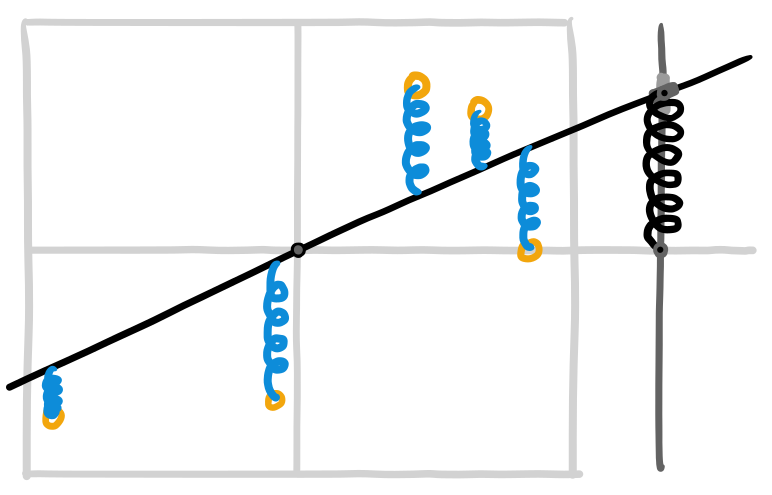
\includegraphics[width=0.99\textwidth]{./regress-springs.png}
  %  \caption{%
  %  \attnsam{caption}
  %  }
  %\end{marginfigure}

  %\begin{marginfigure}[-0cm]
  %  \centering
  %  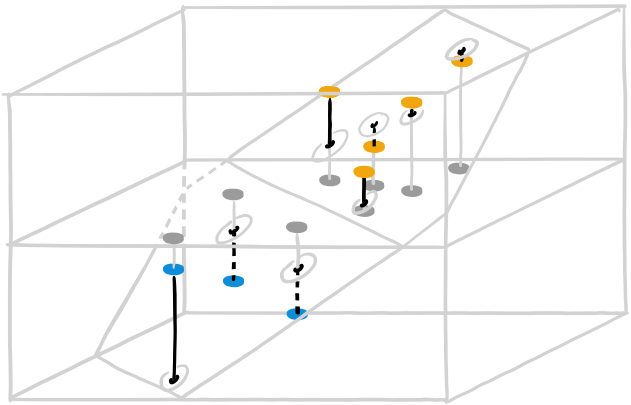
\includegraphics[width=0.99\textwidth]{./regression-beach.png}
  %  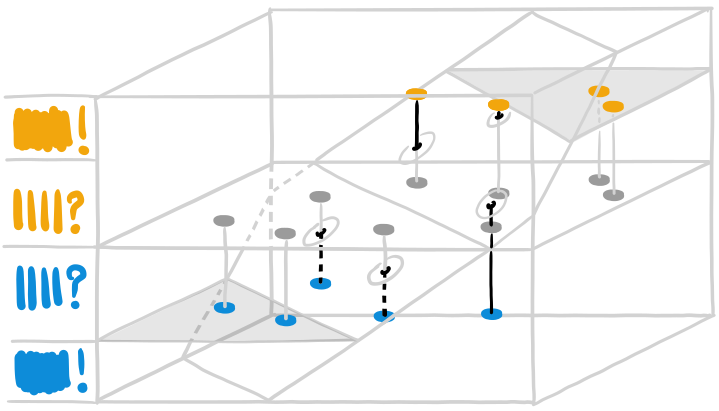
\includegraphics[width=0.99\textwidth]{./hinge-beach.png}
  %  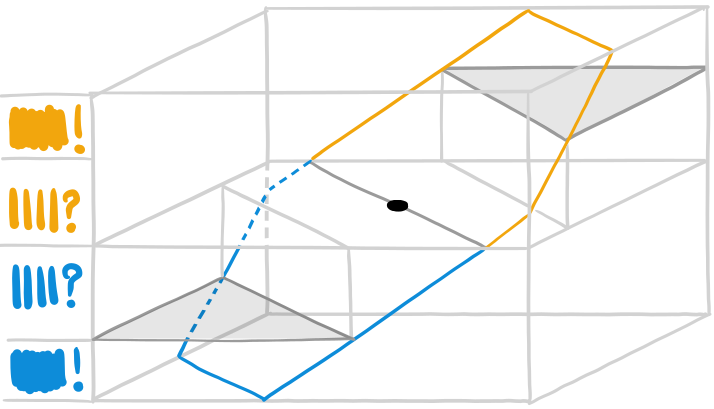
\includegraphics[width=0.99\textwidth]{./beach.png}
  %  \caption{%
  %  \attnsam{caption}
  %  }
  %\end{marginfigure}

        %-- optimization as MAP
        %-- lp priors and sparsity
        %-- generalization as defect of MAP's point estimation (unhumble!)
        %-- pictures of generalization gap vs number of training points
    \samsection{model selection}
      \hypertarget{B3}{}
      %~~~~~~~~~~~~~~~~~~~~~~~~~~~~~~~~~~~~~~~~~~~~~~~~~~~~~~~~~~~~~~~~~~~~~~~~~~~~~~
%~~~~~~~~~~~~~  2.12. taking stock so far  ~~~~~~~~~~~~~~~~~~~~~~~~~~~~~~~~~~~~

      \sampassage{taking stock so far}

%~~~~~~~~~~~~~~~~~~~~~~~~~~~~~~~~~~~~~~~~~~~~~~~~~~~~~~~~~~~~~~~~~~~~~~~~~~~~~~
%~~~~~~~~~~~~~  2.13. grid/random search  ~~~~~~~~~~~~~~~~~~~~~~~~~~~~~~~~~~~~~

      \sampassage{grid/random search}

%~~~~~~~~~~~~~~~~~~~~~~~~~~~~~~~~~~~~~~~~~~~~~~~~~~~~~~~~~~~~~~~~~~~~~~~~~~~~~~
%~~~~~~~~~~~~~  2.14. selecting prior strength  ~~~~~~~~~~~~~~~~~~~~~~~~~~~~~~~

      \sampassage{selecting prior strength}

%~~~~~~~~~~~~~~~~~~~~~~~~~~~~~~~~~~~~~~~~~~~~~~~~~~~~~~~~~~~~~~~~~~~~~~~~~~~~~~
%~~~~~~~~~~~~~  2.15. overfitting on a validation set  ~~~~~~~~~~~~~~~~~~~~~~~~

      \sampassage{overfitting on a validation set}

      \newpage
    \samsection{4. generalization bounds}
      \samquote{
        A foreign philosopher rides a train in Scotland.  Looking out the window,
        they see a black sheep; they exclaim: ``wow!  at least one side of one sheep is black in Scotland!''
      }{unknown}

%~~~~~~~~~~~~~~~~~~~~~~~~~~~~~~~~~~~~~~~~~~~~~~~~~~~~~~~~~~~~~~~~~~~~~~~~~~~~~~
%~~~~~~~~~~~~~  2.16. dot products and generalization  ~~~~~~~~~~~~~~~~~~~~~~~~

      \sampassage{dot products and generalization}
      %\sampassage{perceptron bound}

%~~~~~~~~~~~~~~~~~~~~~~~~~~~~~~~~~~~~~~~~~~~~~~~~~~~~~~~~~~~~~~~~~~~~~~~~~~~~~~
%~~~~~~~~~~~~~  2.17. dimension bound  ~~~~~~~~~~~~~~~~~~~~~~~~~~~~~~~~~~~~~~~~

      %\sampassage{hypothesis-class-based bounds}
      \sampassage{hypothesis-geometry bounds}
        Suppose we are doing binary linear classification with $N$ training
        samples of dimension $d< N$.  Then with probability at least $1-\eta$
        the gen gap is at most:
        %\bcirc\marginnote{%
        %    %\blarr We write $\log_{\!+}(z)$ for $\log(\max(1,z))$.
        %    %\blarr we write $a^\cdot, a^{\cdot\cdot}$ for $(a+1), (a+2)$ to
        %    %avoid overemphasizing annoying constants.
        %}
        $$
          \sqrt{\frac{d\log(6N/d) + \log(4/\eta)}{N}}
        $$
        For example, with $d=16$ features and tolerance $\eta=1/1000$, we
        can achieve a gen.\ gap of less than $5\%$ once we have more than
        $N\approx 64000$ samples.  This is pretty lousy.  It's a worst case
        bound in the sense that it doesn't make any assumptions about how
        orderly or gnarly the data is.

        If we normalize so that $\|x_i\|\leq R$ and we insist on classifiers
        with margin at least $0<m\leq R$, then we may replace $d$ by
        $\lceil 1+(R/m)^2 \rceil$ if we wish, so long as we count each
        margin-violator as a training error, even if it is correctly
        classified.

        \attnsam{CHECK ABOVE!}

        Thus, if $R=1$ and $1 \leq Nm$ then with chance at least $1-\eta$:
        \begin{align*}
            \text{testing error} \leq &~\frac{\text{(number of margin violators)}}{N}
          +\\
            &~\sqrt{\frac{(2/m^2) \log(6N m^2) + \log(4/\eta)}{N}}
        \end{align*}

        \attnsam{dimension/margin}

%~~~~~~~~~~~~~~~~~~~~~~~~~~~~~~~~~~~~~~~~~~~~~~~~~~~~~~~~~~~~~~~~~~~~~~~~~~~~~~
%~~~~~~~~~~~~~  2.18. margin bound  ~~~~~~~~~~~~~~~~~~~~~~~~~~~~~~~~~~~~~~~~~~~

      \sampassage{optimization-based bounds}
        Another way to estimate testing error is through \textbf{leave-one-out
        cross validation} (LOOCV).  This requires sacrifice of a single
        training point in the sense that we need $N+1$ data points to do LOOCV
        for an algorithm that learns from $N$ training points.
        %
       %
        The idea is that after training on the $N$, the
        testing-accuracy-of-hypotheses-learned-from-a-random-training-sample is
        unbiasedly estimated by the learned hypothesis's accuracy on the
        remaining data point.  This is a very coarse, high-variance estimate.
        To address the variance, we can average over all $N+1$
        choices\bcirc\marginnote{%
          \blarr In principle, LOOCV requires training our model $N+1$ many times; we'll
          soon see ways around this for the models we've talked about.
        }
        of which data point to remove from the training set.  When the
        different estimates are sufficiently uncorrelated, this drastically
        reduces the variance of our estimate.

        Our key to establishing sufficient un-correlation lies in
        \emph{algorithmic stability}: the hypothesis shouldn't change too much
        as a function of small changes to the training set; thus, most of the
        variance in each LOOCV estimate is due to the testing points, which by
        assumption are independent.

        If all $x$s, train or test, have length at most $R$, then
        we have that with chance at least $1-\eta$:
        $$
            \Ee_{\sS}
            \text{testing error}
            \leq
            \Ee_{\sS}
            \text{LOOCV error}
            +
            \sqrt{\frac{1+6R^2/\lambda}{2N\eta}}
        $$

        %together with the
        %boundedness and lipschitzness of the ramp function, the LOOCV estimate
        %probably does not severely underestimate the true testing error:
        %$$
        %    \sqrt{\frac{1+6R^2/\lambda}{2N\delta}}
        %    +
        %    \sum_{i} \text{ramp}\left(\frac{\nu^i}{\lambda} \|x^i\|^2 - y^i w\cdot x^i\right)
        %$$


        %% support/sensitiviy bounds
        %Leave-one-out cross-validation gives an unbiased (but not quite
        %1/root n) estimate of generalization gap for N one less than true.
        %%
        %We can proceed further when we're optimizing
        %$$
        %    \lL(w) = \frac{\lambda}{2} \|w\|^2 + \sum_i \ell(-y^i w\cdot x^i)
        %$$
        %where $\ell:\Rr\to\Rr$ is a convex function such as $\text{hinge}$ or
        %$\text{softplus}$.  Suppose that $\ell(d)\geq 0$ and $\ell(d)\to 0$ as
        %its $d\to-\infty$ and $\ell(d)-d \to C$ as $d\to+\infty$ (so slope $1$).

        %The idea is that the optimal $w$ for one less training point shouldn't
        %be that different from the optimal $w$.  If at a training point $i$ we
        %have $d\ell(-y^i w\cdot x^i)/dw$ has norm $\nu^i\|x^i\|$ (largest
        %subgradient--- aka the ``supportiveness of training point i''), then
        %taking out that point shifts $w$ by a distance at most $\nu^i\|x^i\|/\lambda$.
        %So an upper bound for the LOOCV unbiased estimate of the testing
        %error (for N one less) is:
        %$$
        %    \sum_{i} \text{ramp}\left(\frac{\nu^i}{\lambda} \|x^i\|^2 - y^i w\cdot x^i\right)
        %$$
        %where $\text{ramp}(z) = \min(1,\max(0,1+z))$.

%~~~~~~~~~~~~~~~~~~~~~~~~~~~~~~~~~~~~~~~~~~~~~~~~~~~~~~~~~~~~~~~~~~~~~~~~~~~~~~
%~~~~~~~~~~~~~  2.19. bayes and testing  ~~~~~~~~~~~~~~~~~~~~~~~~~~~~~~~~~~~~~~

      \sampassage{bayes and testing}
        % PAC Bayes?  testing Sets?  or maybe testing sets should be part of model selection

      \newpage
    \samsection{5. ideas in optimization}
      \samquote{
        premature optimization is the root of all evil
      }{donald knuth}

        \attn{learning rate as metric; robustness to 2 noise structures}
        \attn{nesterov momentum}
        \attn{decaying step size; termination conditions}
        \attn{batch normalization}



%~~~~~~~~~~~~~~~~~~~~~~~~~~~~~~~~~~~~~~~~~~~~~~~~~~~~~~~~~~~~~~~~~~~~~~~~~~~~~~
%~~~~~~~~~~~~~  2.20. local minima  ~~~~~~~~~~~~~~~~~~~~~~~~~~~~~~~~~~~~~~~~~~~

      \sampassage{local minima}
        % convexity, initialization

%~~~~~~~~~~~~~~~~~~~~~~~~~~~~~~~~~~~~~~~~~~~~~~~~~~~~~~~~~~~~~~~~~~~~~~~~~~~~~~
%~~~~~~~~~~~~~  2.21. implicit regularization  ~~~~~~~~~~~~~~~~~~~~~~~~~~~~~~~~

      \sampassage{implicit regularization}

%~~~~~~~~~~~~~~~~~~~~~~~~~~~~~~~~~~~~~~~~~~~~~~~~~~~~~~~~~~~~~~~~~~~~~~~~~~~~~~
%~~~~~~~~~~~~~  2.22. learning rate schedule  ~~~~~~~~~~~~~~~~~~~~~~~~~~~~~~~~~

      \sampassage{learning rate schedule}

%~~~~~~~~~~~~~~~~~~~~~~~~~~~~~~~~~~~~~~~~~~~~~~~~~~~~~~~~~~~~~~~~~~~~~~~~~~~~~~
%~~~~~~~~~~~~~  2.23. learning rates as dot products  ~~~~~~~~~~~~~~~~~~~~~~~~~

      \sampassage{learning rates as dot products} % connects to whitening / pre-conditioning; ties into next section on kernels

      \newpage
    \samsection{6. kernels enrich approximations}
      \samquote{... animals are divided into (a) those
        belonging to the emperor; (b) embalmed ones; (c) trained ones; (d)
        suckling pigs; (e) mermaids; (f) fabled ones; (g) stray dogs; (h) those
        included in this classification; (i) those that tremble as if they were
        mad; (j) innumerable ones; (k) those drawn with a very fine camel hair
        brush; (l) et cetera; (m) those that have just broken the vase; and (n)
        those that from afar look like flies.
      }{jorge luis borges}

%~~~~~~~~~~~~~~~~~~~~~~~~~~~~~~~~~~~~~~~~~~~~~~~~~~~~~~~~~~~~~~~~~~~~~~~~~~~~~~
%~~~~~~~~~~~~~  2.24. features as pre-processing  ~~~~~~~~~~~~~~~~~~~~~~~~~~~~~

      \sampassage{features as pre-processing} % start with example of (x \mapsto (1, x)) bias trick!

%~~~~~~~~~~~~~~~~~~~~~~~~~~~~~~~~~~~~~~~~~~~~~~~~~~~~~~~~~~~~~~~~~~~~~~~~~~~~~~
%~~~~~~~~~~~~~  2.25. abstracting to dot products  ~~~~~~~~~~~~~~~~~~~~~~~~~~~~

      \sampassage{abstracting to dot products} % mention mercer but don't emphasize

%~~~~~~~~~~~~~~~~~~~~~~~~~~~~~~~~~~~~~~~~~~~~~~~~~~~~~~~~~~~~~~~~~~~~~~~~~~~~~~
%~~~~~~~~~~~~~  2.26. kernelized perceptron and svm  ~~~~~~~~~~~~~~~~~~~~~~~~~~

      \sampassage{kernelized perceptron and svm} % also gaussian process regression?

%~~~~~~~~~~~~~~~~~~~~~~~~~~~~~~~~~~~~~~~~~~~~~~~~~~~~~~~~~~~~~~~~~~~~~~~~~~~~~~
%~~~~~~~~~~~~~  2.27. kernelized logistic regression  ~~~~~~~~~~~~~~~~~~~~~~~~~

     \sampassage{kernelized logistic regression} % leads to nonlinearities...



        %-- featurization
        %-- generalization bounds and BC
        %-- hyperparameter search
        %-- double descent

  \sampart{C. bend those lines to capture rich patterns (units 2,3)}
    \phantomsection\label{part:C}
    \samsection{featurization}
      \hypertarget{C0}{}
      \objectives{%
  \item tailor a hypothesis class by designing features that reflect
        domain knowledge
  \item recognize the geometric patterns that common nonlinear featurizations
        help express
}

%-- what it means for "dogness vs catness" to vary linearly (log probabilities as the thing-to-approximate)
%-- linear geometry of feature space
%-- humble models (svm, perceptron, etc)
%-- featurization and readout //  richer outputs : regression and adt structure

\sampassage{designing featurizations}%\marginnote{\veryoptional}% as an art
%\samquote{%
%  He had bought a large map representing the sea,\\
%  Without the least vestige of land:             \\
%  And the crew were much pleased                 \\
%  when they found it to be                       \\
%  A map they could all understand.
%}{charles dodgson}%
  Remember: our motto in Units 1 and 2 is to \emph{learn linear maps flanked by
  hand-coded nonlinearities}.  That is, we consider hypotheses of this format:
  \[
    \xX                         \xrightarrow[\text{\color{gray}not learned}]{\text{featurize}}
    \Rr^{\# \text{features}}    \xrightarrow[\text{\textbf{learned!}}]{\text{linearly combine}}
    \Rr^{\# \text{outputs}}     \xrightarrow[\text{\color{gray}not learned}]{\text{read out}}
    \yY
  \]
  %
  %where those dimensions $2$ and $1$ more generally count our features and
  %count how many numbers we want to output, respectively.
  %
  In this section and the next we'll design those non-learned functions --- the
  featurizers and readouts, respectively --- to construct a hypothesis class
  $\hH$ suitable given our domain knowledge and our goals.  In this section,
  we'll discuss how the design of features determines the patterns that the
  machine is able to express; feature design can thus make or break an ML
  project.
  %In the next section we'll design readout functions to model uncertainty over
  %$\yY$.

  %\marginnote{%
  %We represent our input $x$ as a fixed-length list of numbers so that we can
  %``do math'' to $x$.  For instance, we could represent a $28\times 28$ photo
  %by $2$ numbers: its overall brightness and its dark part's width.  Or we
  %could represent it by $784$ numbers, one for the brightness at each of the
  %$28\cdot 28=784$ many pixels.  Or by $10$ numbers that respectively measure
  %the overlap of $x$'s ink with that of ``representative'' photos of the digits
  %$0$ through $9$.
  %}

  A way to represent $x$ as a fixed-length list of numbers is a
  \textbf{featurization}.  Each map from raw inputs to numbers is
  a \textbf{feature}.
  %For example, brightness and width are two features.
  %
  %\attnsam{TODO: mention one-hot, etc}
  %\attnsam{TODO: mention LOWRANK (sketching; also, for multiregression)}
  %
  Different featurizations make different
  patterns easier to learn.
  %
  %\marginnote{%
  %    \attnsam{data-based featurizations via kernels}
  %    \attnsam{will soon learn featurizations}
  %    \attnsam{hand featurization in kaggle and medicine}
  %}
  We judge a featurization not in a vacuum but with respect to the kinds of
  patterns we use it to learn. % Good featurizations make task-relevant
  information easy for the machine to use (e.g.\ through apt nonlinearities)
  and throw away task-irrelevant information (e.g. by turning $784$ pixel
  darknesses to $2$ meaningful numbers).
  %\attnsam{TODO: graphic of separability; and how projection can reduce it}

  Here are two themes in the engineering art of featurization.\bovinenote{%
    For now, we imagine hand-coding our features rather
    than adapting them to training data.
    %
    We'll later discuss adapted features; simple examples
    include thresholding into \textbf{quantiles} based on sorted training data (\emph{Is $x$ more than
    the median training point?}), and choosing
    coordinate transforms that measure similarity to \textbf{landmarks}
    (\emph{How far is $x$ from each of these $5$ ``representative'' training
    points?}).  Deep learning is a fancy example.
  }

\sampassage{predicates}
  If domain knowledge suggests some subset
  $S \subseteq \xX$ is salient, then we can define the feature
  $$
    x \mapsto \text{$1$ if $x$ lies in $S$ else $0$}
  $$
  The most important case helps us featurize \emph{categorical} attributes
  (e.g.\ kind-of-chess-piece, biological sex, or letter-of-the-alphabet):
  if an attribute takes $K$ possible values, then each value induces a
  subset of $\xX$ and thus a feature.  These features assemble into a map
  $\xX\to\Rr^K$.  This \textbf{one-hot encoding} is simple, powerful, and
  common.
  %
  Likewise, if some attribute is \emph{ordered} (e.g.\ $\xX$
  contains
      %people and $x<x\pr$ when $x$ descends from $x\pr$.
  geological strata)
  then interesting predicates may include \textbf{thresholds}.
  %
  %\textbf{Binning}.  Conversely, .
  % discrete <--> continuous by softmax, onehot

    %\attnsam{DISTINGUISH BETWEEN TRAINING POINT INDEX vs DIMENSIONS!}

\newpage
\sampassage{coordinate transforms}
    Applying our favorite highschool math functions gives new features
    $
        \tanh(x[0])-x[1],\, |x[1]x[0]| \exp(- x[2]^2),\, \cdots
    $
    from old features $x[0], x[1], \cdots$.
    We choose these functions based on
    domain knowledge; e.g.\ if $x[0], x[1]$ represent two spatial positions,
    then the distance $|x[0]-x[1]|$ may be a useful feature.
    %positions in space, for instance, then we might want
    %    $(x_{20}-x[-])^2 + (x_{21}-x_{1})^2$
    %gives
    %their squared distance.
    %
    One systematic way to include nonlinearities is to include all
    the \textbf{monomials} (such as $x[0] x[1]^2$) with not too many factors ---
    then linear combinations are polynomials.
        %so we call this a \textbf{polynomial featurization}.
    %
    The most important nonlinear coordinate transform uses all monomial
    features with $0$ or $1$ many factors --- said plainly, this maps
    $$
      x \mapsto (1, x)
    $$
    This
    is the \textbf{bias trick}.  Intuitively, it allows the machine to learn
    the threshold above which three-ishness implies a three.
  \begin{marginfigure}[-4cm]
    \centering
    \picturew{0.99\textwidth}{bias-trick}
    \caption{%
        %\textsc{Above}:
        \textbf{The bias trick helps us model `offset' decision boundaries.}
        Here, the origin is the lower right corner closer to the camera.  Our
        raw inputs $x=(x[0],x[1])$ are $2$-D; we can imagine them
        sitting on the bottom face of the plot (bottom ends of the vertical
        stems).  But, within that face, no line through the origin separates
        the data well.  By contrast, when we use a featurization
        $(1,x[0],x[1])$, our data lies on the top face of the plot; now a plane
        through the origin (shown) successfully separates the data.
        %
        %\\
        %\textsc{Below}:
    }
  \end{marginfigure}

  This bias trick is non-linear in that it shifts the origin.  Fancier
  non-linearities enrich our vocabulary of hypotheses in fancier ways.  Take a
  look these decision boundaries using a degree-$2$ monomial feature (left) and
  (right) a non-polynomial `black hole' feature for two cartoon datasets:
  \begin{figure}[h]
    \centering
    \picturew{0.45\textwidth}{quadratic-features}%
    \picturew{0.48\textwidth}{black-hole}%
    \caption{%
      \textbf{Fancier nonlinearities help us model curvy patterns using linear weights.}
      \textbf{Left}:
      Using a quadratic feature (and the bias trick, too) we can
      learn to classify points in $\xX=\Rr^1$ by whether they are in some
      \emph{interval} {\textbf{\dgre gray region}}.  We don't know the interval
      beforehand, but fortunately, different linear decision boundaries
      (\textbf{black lines}) in feature-space give rise to \emph{all possible}
      intervals!  We may optimize as usual to find the best interval.
      %
      %%You might say: \emph{why sweat through all that work
      %%with polynomials when we could just describe the intervals directly?}.
      %%Answer: real-world data is high-dimensional and we often want to capture
      %%patterns trickier than intervals.  Polynomials and other smooth functions
      %%make modeling high-dimensional patterns almost as easy as modeling
      %%intervals.  We'll especially see this in Unit 3.
      %
      \\
      \textbf{Right}:
      No line through $\xX=\Rr^2$ separates our raw data.  But a
      \textbf{(black) hyperplane} \emph{does} separate our featurized data.  We
      are thus able to learn a hypothesis that predicts the {\blu blue} label
      for $x$s inside the {\textbf{\dgre gray region}}.
      Intuitively, the `black hole' feature measures whether an input $x$ is
      nearby a certain point in $\xX$.
      %
      \exercise{%
        Our `black hole' decision boundary actually has two parts, one
        finite and one infinite.  The infinite part is slightly `off-screen'.
        Sketch the full situation out!
      }
    }
  \end{figure}
  \begin{marginfigure}[+4cm]
    \centering
    \picturew{0.70\textwidth}{satellite-2}%
  \end{marginfigure}

  Say $\xX=\Rr^2$ has as its two raw features the latitude of low-orbit
  satellite and the latitude of a ground-based receiver, measured in
  degrees-from-the-equator.  So the satellite is in earth's north or southern
  hemisphere and likewise for the receiver.  We believe that whether or not the
  two objects are in the \emph{same} hemisphere --- call this situation
  `visible' --- is highly relevant to our ultimate prediction task.
  \exercise{%
    For practice, we'll first try to classify $x$s by visibility.
    %
    Define a degree-$2$ monomial feature $\varphi:\xX\to \Rr^1$ whose sign
    ($\pm 1$) tells us whether $x$ is visible.\bovinenote{%
      Thus, degree-$2$ monomials help model $2$-way interactions
      between features.
      %Likewise for higher degres.
    }
    %
    \emph{Can direct linear use of $x$, even with the bias trick, predict the
  same?}
  }
  \par\noindent
  In reality we're interested in a more complex binary classification task on
  $\xX$.  For this we choose as features all monomials of degrees $0,1,2$ to
  get $\varphi:\xX\to\Rr^6$.\bovinenote{%
    \noparexercise{%
      $\varphi$ maps to $\Rr^6$, i.e., we have exactly $6$ monomials.  Verify this!
    }
  }
  \exercise{%
    %
    Qualitatively describe which input-output rules $h:\xX\to\{+1,-1\}$ we can
    express.  For
    instance, which of these rules in the margin\bovinenote{%
      \textsc{Rule A}
        ``{$+1$ exactly when the satellite is between the Tropics of Cancer and of Capricorn}''
      \textsc{Rule B}
        ``{$+1$ exactly when satellite and receiver are at the same latitude, up to $3^\circ$ of error}''
      \textsc{Rule C}
        ``{$+1$ exactly when both objects are above the Arctic Circle}''
        }
    can we express?
    (Formally, we can `express' $h$ if
    $h(x)=\text{sign}(w\cdot \varphi(x))$ for some $w$.)
  }
  \par\noindent

\newpage
\sampassage{interpreting weights}
  The features we design ultimately get used
  according to a weight vector.
  So we stand to gain from deeper understanding of what weights `mean'.
  Here we'll discuss three aspects of the `intuitive logic' of weights.

  First, \textbf{weights are not correlations}.
  %
  A feature may correlate with a positive label ({say, $y={\blu +1}$})
  yet fail to have a positive weight.
  %coefficient in an optimal weight vector.
  That is: the \emph{blah}-feature could correlate with $y={\blu +1}$ in the
  training set and yet, according to the best hypothesis for that
  training set, the bigger a fresh input's \emph{blah} feature is, the
  \emph{less} likely its label is to be ${\blu +1}$, all else being equal.
  That last phrase ``all else being equal'' is crucial, since it refers to our
  choice of coordinates.

  In Figure \ref{fig:interpreting-weights}'s center-left panel, the weight for brightness is negative
  even though both features positively correlate with {\blu blue}!  This is
  because brightness correlates \emph{even better} with the
  \emph{error} of soley-width-based prediction.  So the
  optimal hypothesis, intuitively, uses the brightness as a `correction'
  to width.
  %
  This contrasts with the top-left panel, where the both correlations are still
  positive and both weights are positive.  Intuitively,
  the optimal hypothesis here reduces noise by averaging a solely-brightness-based
  prediction with a solely-width-based one.

  \begin{marginfigure}[-.6cm]
    \centering
    \picturew{0.99\textwidth}{depshear}%
    \caption{%
      \textbf{Relations between feature statistics and optimal weights.}
      Each panel shows a different 2D binary classification task
      and a maximum-margin hypothesis.  We shade margin-achieving points.
      To save ink we refer to the vertical and horizontal features
      as \textbf{brightness} and \textbf{width};
      but you should be more imaginative.
      %In these examples, \emph{optimal}
      %means ``achieves minimal training error, even if we jiggle the training
      %points a bit''.  That is, we want the dividing line to be as far from
      %the training points as possible, so that small jiggles don't lead to
      %misclassifications.  Intuitively, testing points are jiggled versions of
      %training points, so this seems like a reasonable criterion.  Later we'll
      %see how this arises from theory.
      %---
      \textbf{Left:} \emph{positive weights are consistent with positive, negative,
      or zero correlation!}
      %---
      \textbf{Right:}  \emph{presenting the same information in different
      coordinates (here, all 2D) alters predictions!}
      \exercise{%
        Think of
        classification tasks (and feature-pairs) that could
        plausibly give rise to the data depicted in each panel.
        %the depicted data.
      }
    }
    \label{fig:interpreting-weights}
  \end{marginfigure}

  %\attnsam{Note on interpreting weights}
  %% dependence

  Second, \textbf{representing the same information two different ways can alter
  predictions}.  A featurization doesn't just supply raw data: it
  also suggests to the machine which patterns are possible and, among those,
  which are plausible.

  The bias trick and other nonlinear coordinate transforms illustrate this.
  % shearing
  But even \emph{linear}, origin-preserving coordinate-transforms can alter
  predictions.
  For example, if we shear two features together --- say, by using
  $\{$preptime-plus-cooktime and cooktime$\}$ as features rather than
  $\{$preptime and cooktime$\}$ --- this can impact the decision boundary.
  %
  Of course, the decision boundary will look different because we're in
  new coordinates; but we mean something more profound:
    if we train in old coordinates and then predict a datapoint represented in old coordinates,
  we might get a different prediction than
    if we train in new coordinates and then predict a datapoint represented in new coordinates!
  %
  See the right three panels:
  the intersection of the two {\gre gray lines} implicitly marks
  a testing point for which we predict different labels
  as we
  change
  %adopt different
  coordinates.
  %
  \emph{Intuitively, the more stretched out a feature axis is, the more the
  learned hypothesis will rely on that feature.}\bovinenote{%
    \noparexercise{%
      Explain the preceding intuition in terms of the L2 regularizer.
    }
  }

  Third, \textbf{features interact}.
  It's useful to think about `the goodness' of individual features,
  but it's also good to realize that the reality is messier: a feature's
  predictive usefulness depends on which other features are present!

  That is, a whole can be more (or less!) than the sum of its parts: the
  usefulness of a set of features ain't `additive' the way the weight of a set
  of books is.  Here's a simple example: let's flip two fair coins.  We want to
  predict whether they ended up the same or not.  Knowing the value of just the
  first coin is totally useless to prediction!  Same with the value of just the
  second coin.  BUT the two coins together help us predict 100\% correctly.\bovinenote{%
    \noparexercise{%
      Find an analogue of the coins story where the whole
      is less than the sum of its parts, predictivity-wise.
    }
  }
  Likewise, in the bottom-left panel the width is \emph{independent} of the
  class label but not \emph{conditionally-independent}-given-brightness.
  %
  It's this that explains why we can't just compute the correlation of each
  feature with the predictand and then call it day.






        %-- linear preprocessing (emphasis; feature extraction and pca)
        %-- kernels enrich approximations
        %-- decision trees, polynomials, binning, and other nonlinear ideas
        %-- random sketching
    \samsection{learned featurizations}
      \hypertarget{C1}{}
      %\samsection{1. learned featurizations}
\sampassage{imagining the space of feature tuples}
  We'll focus on an architecture of the form
  $$
    \hat p(y\!=\!+1\,|\,x) \,=\,
    (\sigma_{1\times 1} \circ
    A_{1\times (h+1)} \circ
    f_{(h+1)\times h} \circ
    B_{h\times d})(x)
  $$
  where $A,B$ are linear maps with the specified
  $(\text{input}\times\text{output})$ dimensions, where $\sigma$ is the
  familiar sigmoid operation, and where $f$ applies the leaky relu
  function elementwise and concatenates a $1$:
  $$
    f((v_i : 0\leq i<h)) = (1,)\,+\!\!\!\!+\,(\text{lrelu}(v_i) : 0\leq i<h)
    \quad \quad
    \text{lrelu}(z) = \max(z/10, z)
  $$
  We call $h$ the \textbf{hidden dimension} of the model.
  %
  Intuitively, $f \circ B$ re-featurizes the input to a form more
  linearly separable (by weight vector $A$).

\sampassage{the featurization layer's learning signal}
\sampassage{expressivity and local minima}% approximation % logic, etc
\sampassage{``representer theorem''}



        %-- one hidden layer ; activ.s/pools/flows as creative engineering
        %-- fancier gradient-based methods (nesterov, adam, etc)
        %-- multi-layer and skip connections : width vs depth
        %-- hierarchical features appear
    \samsection{locality and symmetry in architecture}
      \hypertarget{C2}{}
          \samsection{2. multiple layers}
        We can continue alternating learned linearities with fixed
        nonlinearities:
        \begin{align*}
          \hat p(y\!=\!+1\,|\,x) \,=\,
          (\sigma_{1\times 1} \,\circ\,
          A_{1\times (h\prpr +1)} \,\circ\,
            &f_{(h\prpr+1) \times h\prpr} \,\circ\,
          B_{h\prpr \times (h\pr+1)} \,\circ\, \\
            &f_{(h\pr+1)\times h\pr} \,\circ\,
          C_{h\pr\times (h+1)} \,\circ\, \\
            &f_{(h+1)\times h} \,\circ\,
          D_{h\times d})(x)
        \end{align*}

      \sampassage{feature hierarchies}
      \sampassage{bottlenecking}
      \sampassage{highways}
      %\sampassage{differentiation} % addressed in 0.

    \samsection{3. architecture and wishful thinking}
      \sampassage{representation learning} % leads to lstms etc

    \samsection{4. architecture and symmetry} % and other priors?
      \samquote{
        About to speak at [conference].  Spilled Coke on left leg of jeans, so
        poured some water on right leg so looks like the denim fade.
      }{tony hsieh}



        %-- convolutions
        %-- attention and transformers
        %-- gnns
        %-- survey of approaches to symmetry
    \samsection{dependencies in architecture}
      \hypertarget{C3}{}
          \samsection{5. stochastic gradient descent}
      \samquote{
        The key to success is failure.
      }{michael j.\ jordan}

    \samsection{6. loss landscape shape}
      \samquote{
        The virtue of maps, they show what can be done with limited space, they
        foresee that everything can happen therein.
      }{jos\'e saramago}

        %-- siamese and masked nets
        %-- rnns (also philosophy of ntms and stack lstms?)
        %-- autoencoders
        %-- "downstream" representation learning

  \sampart{D. thicken those lines to quantify uncertainty (unit 4)}
    \phantomsection\label{part:D}
    \samsection{bayesian models}
      \hypertarget{D0}{}
      \input{tex-source/body.3.0.bayesian-models}
        %-- example; graphical notation
        %-- explaining away and the forward-backward flow of information
        %-- the `logic` of probability
        %-- hierarchy and transfer
    \samsection{examples of bayesian models}
      \hypertarget{D1}{}
      \input{tex-source/body.3.1.examples-of-bayesian-models}
        %-- gmms for clustering ; limit of k-means
        %-- hmms
        %-- fonts, glyphs, occlusion (rendering)
        %-- feras time-series-from-programs
    \samsection{inference algorithms for bayesian models}
      \hypertarget{D2}{}
      \input{tex-source/body.3.2.inference-algorithms-for-bayesian-models}
        %-- variational : expectation maximization
        %-- more on variational : expectation maximization
        %-- sampling : hmmcmc
        %-- more on sampling : hmmcmc
    \samsection{combining with deep learning}
      \hypertarget{D3}{}
      \input{tex-source/body.3.3.combining-with-deep-learning}
        %-- neural nets for amortized inference
        %-- variational autoencoders
        %-- richer probabilistic outputs
        %-- analysis by synthesis

  \sampart{E. beyond learning-from-examples (unit 5)}
    \phantomsection\label{part:E}
    \samsection{reinforcement ; bandits}
      \hypertarget{E0}{}
      \input{tex-source/body.4.0.reinforcement}
    \samsection{state (dependence on prev xs and on actions ) ; RL ; partial observations}
      \hypertarget{E1}{}
      \input{tex-source/body.4.1.state}
    \samsection{deep q learning}
      \hypertarget{E2}{}
      \input{tex-source/body.4.2.deep-q-learning}
    \samsection{learning-from-instructions ; farewell}
      \hypertarget{E3}{}
      \input{tex-source/body.4.1.learning-from-instructions}

  %\sampart{F. appendices (unit 0; LOW PRIORITY; assemble from old piazza posts)}
  % \phantomsection\label{part:F}
  %  \samsection{probability primer}
  %   \hypertarget{F0}{}
  %    
    \samsection{probability and generalization}%, independence, concentration}
      \samquote{
        Can I just say Chris for one moment that I have a new theory about the
        brontosaurus. ...  This theory goes as follows and begins now. All
        brontosauruses are thin at one end, much, much thicker in the middle
        and then thin again at the far end. That is my theory, it is mine, and
        belongs to me and I own it, and what it is too.
      }{john cleese}

      \sampassage{belief and bayes}
      \sampassage{the key abstraction: averages}
      \sampassage{the key approximation: independence}
      \sampassage{uniform concentration}


  %      %-- fundamentals; frequentism vs bayesianism
  %      %-- 2 sharp tools: independence and averaging
  %      %-- log loss and friends
  %      %-- common families of distributions
  %  \samsection{linear algebra primer}
  %   \hypertarget{F1}{}
  %    
    \samsection{linear algebra and approximation}
      \samquote{
        Stand firm in your refusal to remain conscious during algebra.
        In real life, I assure you, there is no such thing as algebra.
      }{fran lebowitz}

        Linear algebra is the part of geometry that focuses on when a point is
        the origin, when a `line' is a straight, and when two straight lines
        are parallel.
        %
        Linear algebra thus helps us deal with the preceding pictures
        mathematically and automatically.  The concept of `straight lines'
        gives a simple, flexible model for extrapolation from known points to
        unknown points.  That is intuitively why linear algebra will be crucial
        at every stage of 6.86x.

      \sampassage{visualizing high dimensional spaces}
      \sampassage{column vectors and row vectors} % vectors and co-vectors
        The elements of linear algebra are \textbf{column vectors} and
        \textbf{row vectors}.\bcirc \marginnote{%
          \blarr Though we represent the two similarly in a computer's memory, they
          have different geometric meanings.  We save much anguish by
          remembering the difference.
        }
        We have a set $V$ of ``column vectors''.  We're allowed to find $V$'s
        zero vector and to add or scale vectors in $V$ to get other vectors in
        $V$.  $V$ is the primary object we hold in our mind; perhaps, if we're
        doing image classification, then each column vector represents a
        photograph.  We use the word ``space'' or ``vector space'' when talking
        about $V$ to emphasize that we'd like to exploit visual intuitions when
        analyzing $V$.  In short: we imagine each column vector as a point in
        space, or, if we like, as an arrow from the zero vector to that point.

        Now, associated to $V$ is the set of ``row vectors''.  Under the hood, a
        row vector is a linear function from $V$ to the real numbers $\Rr$.  We
        imagine each row vector not as an arrow but as a ``linear'' heat map or
        altitude map that assigns to each point in $V$ a numeric ``intensity''.
        We can visualize a row vector the same way makers of geographic maps
        do: using contours for where in $V$ the row vector attains values
        $\cdots,-2,-1,0,+1,+2,\cdots$.
        These will be a bunch of uniformly spaced parallel ``planes''.  The
        spacing and orientation of the planes depends on and determines the row
        vector.  In short, we imagine each row vector as a collection of
        parallel planes in space.

        Informally: a column vector is a noun or thing whereas a row vector is
        a adjective or property.  The degree to which a property holds on a
        thing (or a description is true of a thing) is gotten by evaluating the
        row vector on the column vector --- remember, a row vector is a
        function, so we can do this evaluation.  Geometrically, if a row vector
        is a bunch of planes and a column vector is an arrow, the two evaluate
        to a number: the number of planes that the arrow pierces.  Intuitively,
        an example of a column vector might be ``this particular photo of my
        pet cow''; an example of a row vector might be ``redness of the left
        half (of the input photo)''.  If we evaluate this row vector on this
        column vector, then we get a number indicating how intensely true it is
        that the left half of that particular photo is red.\marginnote{%
            We can draw an analogy with syntax vs semantics.  This pair of
            concepts pops up in linguistics, philosophy, circuit engineering,
            quantum physics, and more, but all we need to know is that:
            semantics is about things while syntax is about descriptions of
            things.  The two concepts relate in that, given a set of things, we
            can ask for the set of all descriptions that hold true for all
            those things simultaneously.  And if we have a set of descriptions,
            we can ask for the set of all things that satisfy all those
            descriptions simultaneously.  These two concepts stand in formal
            opposition in the sense that: if we have a set of things and make
            it bigger, then the set of descriptions that apply becomes smaller.
            And vice versa.  Then a column vector is an object of semantics.
            And a row vector is an object of syntax.
        }

      \sampassage{inner products}
        Now, here is the key point: the engine behind generalization in machine
        learning (at least, the machine learning we'll do in Units 1 and 2; and
        less visibly but still truly in more than half of each of Units 3,4,5)
        is the ability to translate between things and properties.  If ``my pet
        cow'' is a thing, then ``similar to my pet cow'' is a property.  The whole
        project of machine learning is to define and implement this word
        ``similar to''.  When we define and implement well, our programs can
        generalize successfully from training examples to new, previously
        unseen situations, since they will be able to see which of the training
        examples the new situations are similar to.  Since ``similar to''
        transforms things to properties, the linear algebra math behind
        ``similar to'' is a function from column vectors to row vectors.  This
        brings us to...

        ... inner products, aka kernels.  An inner product is just a fancy word
        for a (linear) function from column vectors to row vectors.  We
        actually demand that this linear function has two nice properties:
        FIRST, it should have an inverse.  That is, it ought to be a two way
        bridge between column vectors and row vectors, allowing us to translate
        things to descriptions and vice versa.  SECOND, it should be symmetric.
        This means that if we have two things, say ``my pet cow'' and ``my pet
        raccoon'', then the degree to which ``my pet raccoon'' has the property
        ``is similar to my pet cow'' ought to match the degree to which ``my pet
        cow'' has the property ``is similar to my pet raccoon''.  Any invertible,
        symmetric, linear function from column vectors to row vectors is called
        an inner product.  Kernel is a synonym here.\marginnote{%
          Beware: the same word, ``kernel'', has different meanings depending
          on context.
        }

        There are generally infinitely many inner products.  Which one we
        choose changes the generalization properties of our machine learning
        program.  Practically, if we are doing machine learning in a concrete
        situation, then we want to choose an inner product that reflects our
        human intuition and experience and domain knowledge about the right
        notion of ``similarity'' in that situation.

        Any inner product $P$ from column vectors to row vectors induces notions
        of length and angle.  We just define a column vector v's length by
        $\sqrt{P(v)(v)}$.  Call that quantity $\|v\|$.  And we define the angle
        $\alpha(v,w)$ between two non-zero column vectors v,w by
        $P(v)(w)=\|v\|\cdot\|w\|\cdot\cos\alpha(v,w)$.  We make these
        definitions so as to match the Pythagorean theorem from plane geometry.\marginnote{%
          You can google up proofs of the Pythagorean theorem (many are quick and
          beautiful) if you wish to dig deeper.
        }
        So once we choose which inner product we'll use (out of the infinitely
        many choices), we get the concepts of euclidean geometry for free.
        Immediately following from that definition of angle, we get that if two
        column vectors have vanishing inner product (i.e., if $P(v)(w)=0$), then
        those vectors are at right angles (i.e. $\alpha(v)(w)=\pi/2$).

        Now, sometimes (but most of the time not), we are blessed in
        that we know more about our situation than just the space V of things.
        Specifically, V might come with a canonical basis.  This just means
        that V comes marked with "the right" axes with respect to which we
        ought to analyze vectors in V.  In this fortunate case, there is also a
        canonical inner product.  It's called dot product.  Again, I want to
        emphasize that a plain vector space doesn't come with a dot product.
        We need a basis for that.

        The dot product is defined as follows.  Say there are $D$ axes and that
        the "unit" vectors along each axis (aka the basis vector) are named
        $(v_i:0\leq i<D)$.  Then we define $P(v_j)(v_i) = (1 \text{ if } i=j
        \text{ else } 0)$ --- the $1$ expresses that each "unit" basis vector
        ought to have length $1$.  The $0$ expresses that different basis
        vectors ought to be at right angles to each other.  This determines $P$
        on all inputs, by linearity: $P(\sum c^\pr_j v_j)(\sum c_i v_i)=\sum_i
        c^\pr_i c_i$ where $c^\pr_j,c_i$ are numbers.  In short: given a basis,
        there is a unique inner product such that those basis elements all have
        length $1$ and are at right angles to each other.  We call that inner
        product the dot product.

        \attnsam{FILL IN LINEAR DECISION BOUNDARY! (remark on featurization and
        argmax nonlinearities)}

        We may \textbf{evaluate} a row vector on a column vector.  \attnsam{FILL
        IN} A \textbf{dot product} is a way of translating between row and
        column vectors.  \attnsam{FILL IN: DISCUSS GENERALIZATION; (DISCUSS ANGLE, TOO)}

      \sampassage{linear maps}

      \sampassage{singular value decomposition}



  %      %-- linear "spaces" and linear "maps"
  %      %-- dimension, trace, determinant, visually
  %      %-- vectors, covectors, higher tensors
  %      %-- dot product, angles, and svd, visually
  %  \samsection{derivatives primer}
  %   \hypertarget{F2}{}
  %    
    \samsection{calculus and optimization}%gradients
      \samquote{
        The self is not something ready-made, but something in continuous
        formation through choice of action.
      }{john dewey}

      Throughout this section, $X$ and $Y$ will refer to two normed real
      vector spaces of finite dimension.

      \sampassage{asymptotic notation}
        When analyzing algorithms or data, we often wish to consider extremes
        of the very small or the very large.  Such thought experiments isolate
        how behaviors of interest depend on the variables we take to extreme
        values.

        We say \textbf{$f:X\to Y$ is negligible compared to $g:X\to Y$
        for sufficiently small\bovinenote{%
          The notion that ``\emph{$f$ is negligible compared to $g$ for
          sufficiently small inputs}'' is the most important of a $2\times 2$
          grid of variants:
          we may change
          $$\text{sufficiently small} \rightsquigarrow \text{sufficiently large}$$
          by replacing
          $$\text{``$0<\|x\|<\delta$''} \rightsquigarrow \text{``$\delta<\|x\|$''}$$
          and/or we may change
          \begin{align*}
              &\text{is negligible compared to}\\
              \rightsquigarrow~
              &\text{never overwhelms}
          \end{align*}
          by replacing
          \begin{align*}
              &\text{``For any positive number $\epsilon$''}\\
              \rightsquigarrow~
              &\text{``There exists a positive number $\epsilon$''}
          \end{align*}
          %
          The class of $f$s that never ovewhelm $g$ is called $O(g)$ --- pronounced
          \textbf{big-Oh}.  Clearly, $o(g) \subsetneq O(g)$.
          Confusingly, folks use the same notation $o(g), O(g)$
          when considering small inputs and large inputs;
          which sense we mean should be clear from context.
        } inputs}
        when the ratio $\|f\|/\|g\|$ is tiny for small inputs --- that is, when:
        \begin{align*}
            &\hspace{0cm}\text{For any positive number $\epsilon$}\\
            &\hspace{1cm}\text{there exists a positive number $\delta$ so that,}\\
            &\hspace{2cm}\text{whenever $0<\|x\|<\delta$,}\\
            &\hspace{3cm}\text{we also have $\|f(x)\| < \epsilon \|g(x)\|$.}
        \end{align*}
        The class of $f$s that are negligible compared to $g$ we denote by
        $$
            o(g)
        $$
        or, when abusing notation, by $o(g(x))$ even though $x$
        isn't defined.  This is \textbf{little-oh} notation.

        For example, if $p,q$ are positive real numbers
        then $|x|^p$ is negligible compared
        to $|x|^q$ if and only if $p<q$:
        $$
            (x \mapsto |x|^3)     \in o(x \mapsto |x|^2)
            \quad\quad
            (x \mapsto |x|^3) \not\in o(x \mapsto |x|^4)
        $$

        \par\noindent
        \attn{Exercise:} {Is $\sin(x) \in o(1)$?  How about $o(x)$?}

        \par\noindent
        \attn{Exercise:} {Is $\max(0,x) \in o(1)$?  How about $o(x)$?}

        \par\noindent
        \attn{Exercise:} {Is $\log |x| \in o(1/x)$?  (Ignore $x=0$.)}

        \par\noindent
        \attn{Exercise:} {Is $\exp(-1/|x|) \in o(x)$?  (Ignore $x=0$.)}

      \sampassage{derivatives}
        If $f:X\to Y$ is a (potentially nonlinear) function between two
        finite-dimensional real vector spaces, we may wish to approximate $f$
        by a linear function (plus a constant).  It is often unreasonable to
        ask that the approximation is good for all inputs; instead, we ask that
        the approximation is good near some specific input $x:X$:
        $$
            f(x+h) \approx f(x) + (Df_x)(h)
        $$
        Here, $(Df_x):X\to Y$ is a linear map that translates changes $h$ in
        $f$'s input to changes $(Df_x)(h)$ in $f$'s output.  We want the
        approximation to be good for small $h$ in the sense that the error
        vanishes faster than linearly as $h$ shrinks:
        $$
            \|f(x) + (Df_x)(h) - f(x+h)\| \in o(\|h\|)
        $$
        Intuitively, $Df_x$ exists when $f$ varies smoothly.

      \sampassage{integrals}
      \sampassage{}



  %      %-- derivatives are best linear appro.s: chain rule and linearity
  %      %-- product rule, visually
  %      %-- optimization : critical points, lagrange, higher derivatives
  %      %-- write your own automatic differentiator: a short exercise
  %  \samsection{programming and numpy and pytorch primer}
  %   \hypertarget{F3}{}
  %    
%==============================================================================
%====  7.  PROGRAMMING REFRESHER  ============================================
%==============================================================================

  \newpage
  \sampart{G. (python) programming refresher}\label{chap:programming}

    \samsection{python setup}
      \samquote{
        If I have not seen as far as others, it is because giants were standing
        on my shoulders.
      }{hal abelson}

      \sampassage{what's python?}
        Python is a programming language.  Its heart is the
        \textbf{Python interpreter}, a computer program that takes a plain
        text file such as this two-liner\bcirc\marginnote{%
          \blarr The instruction \texttt{print} just displays some text
          onto our screen.  For example, the first line of this program
          displays \texttt{hello, world!} onto our screen.  This instruction
          doesn't rely on or activate any ink-on-paper printing machines.
        } ---
        \begin{lstlisting}[language=Python, basicstyle=\footnotesize\ttfamily]
          print('hello, world!')
          print('cows and dogs are fluffy')
        \end{lstlisting}
        --- and executes the instructions contained in that text file.  We
        call these textual instructions are \textbf{source code}.

        The instructions have to be in a certain, extremely rigid format in
        order for the interpreter to understand and execute them.  That's why
        they call Python a \emph{language}: it has its own rigid grammar
        and its own limited vocabulary.  If the
        interpreter encounters incorrectly formatted instructions --- if even a
        single punctuation mark is missing or a --- the interpreter will display a
        bit of text in addition to the word \texttt{Error} and immediately
        after abort its mission.\bcirc\marginnote{%
          \blarr Adventure boldly when learning Python!  It might feel
          catastrophic when you encounter an error and the interpreter
          `dies'.  But (unless you go out of your way to use special
          instructions we won't teach in class) these errors won't hurt your
          computer.  There aren't any lasting effects.
          %
          So \textbf{errors are hints, not penalties}.
          If you encounter an
          error, just modify your instructions to address that error, then run
          the interpreter again.
          %
          Engage in a fast feedback cycle (\emph{I'll try this... error...
          okay how about this...  different error... hmm let's think...})
          to learn to program well.
        }

        We'll use Python in 6.86x to instruct our computer to analyze data.
        The gigantic project of instructing a computer is a bit like teaching a
        person by mail.  We never see them; we exchange only written words.
        They have never seen a horse, and yet we want to teach them to
        distinguish horses from zebras from donkeys from tapirs from rhinos.
        Though severely limited in their vocabulary and their ability to
        appreciate analogies and similarities, they are extraordinarily
        meticulous, patient, and efficient.
        %
        That's what programming will be like.

        At this point, you might have several questions:
        \begin{description}
          \item[\textbf{Picking up the pen:}] How do I install and use the Python
               interpreter?
          \item[\textbf{Writing sentences:}] What syntax rules must my
               instructions obey in order for the interpreter to understand
                that I want it do such-and-such task?
          \item[\textbf{Composing essays:}] How do I organize large programs?
          \item[\textbf{Teaching via mail:}] What instructions
               make the computer analyze data?
        \end{description}
        This and the next three sections address these four
        questions in turn.

      \sampassage{which things we'll set up}
        Let's set up Python by installing the Python interpreter.
        %
        Actually, I should say \emph{a} Python interpreter: each of the many
        software tools we'll use in 6.86x has a zillion versions; it can get
        confusing tracking which versions coexist and which clash.  We will use
        \textbf{Python version 3.8} throughout 6.86x.

        Beyond the Python interpreter, there is an ecosystem of useful tools:
        machine learning modules that help us avoid reinventing the wheel; a
        rainbow of feature-rich text editors specialized for writing Python code;
        and a package manager called \texttt{conda} that eases the logistics
        nightmare of coordinating the versions we have of each tool.

      \sampassage{setup on windows}
        \attnsam{Mohamed, please fill this out}
        \attnsam{(mention windows 10 and higher's `linux subsystem?')}

      \sampassage{setup on macOS}
        \attnsam{Karene, please fill this out}

      \sampassage{setup on linux}
        I'll assume we're working with Ubuntu 20.04.  If you're on a
        different Linux, then similar steps should work --- google search to
        figure out how.

      \sampassage{checking the setup}
        Let's create a new plain text file containing this single line:\bcirc\marginnote{%
          \blarr This line contains \textbf{Python source code}.  When we include
          Python source code in these notes, we will format it for readability,
          e.g.\ by making key parts of it bold.  However, this depiction of
          source code is supposed to represent \emph{plain text}.
        }
        \begin{lstlisting}[language=Python, basicstyle=\footnotesize\ttfamily]
          print('hello, world!')
        \end{lstlisting}
        We can name the file whatever we want --- say, \texttt{greetings.py}.
        Then in your terminal (navigate to the same directory as the file and)
        enter this command:
        \begin{lstlisting}[basicstyle=\footnotesize\ttfamily]
          python3 greetings.py
        \end{lstlisting}
        A new line should appear in your terminal:
        \begin{lstlisting}[basicstyle=\footnotesize\ttfamily]
          hello, world!
        \end{lstlisting}
        After that line should be another shell prompt.

        Now append three lines to the file \texttt{greetings.py} so that its
        contents look like:
        \begin{lstlisting}[language=Python, basicstyle=\footnotesize\ttfamily]
          print('hello, world!')
          fahr = int(input('please enter a number... '))
          celc = int((fahr - 32.0) * 5.0/9.0)
          print('{} fahrenheit is roughly {} celcius'.format(fahr, celc))
        \end{lstlisting}
        Again, enter the following command in your terminal:
        \begin{lstlisting}[basicstyle=\footnotesize\ttfamily]
          python3 greetings.py
        \end{lstlisting}
        Two new lines should appear in your terminal:
        \begin{lstlisting}[basicstyle=\footnotesize\ttfamily]
          hello, world!
          please enter a number...
        \end{lstlisting}
        Enter some number --- say, $72$; a new line should appear in your
        terminal so that the overall session looks something like:
        \begin{lstlisting}[basicstyle=\footnotesize\ttfamily]
          hello, world!
          please enter a number... 72
          72 fahrenheit is roughly 22 celcius
        \end{lstlisting}
        After that line should be another shell prompt.

        If you did the above but something different from the predicted lines
        appeared, that means something is amiss with Python setup.  Please let
        us know in this case!  We can try to help fix.


    \samsection{elements of programming}
      \samquote{
        Displace one note and there would be diminishment, displace one phrase
        and the structure would fall.
      }{antonio salieri, on wolfgang mozart's music, as untruthfully portrayed in \emph{Amadeus}}

        %% use-mention distinction; syntax-semantic.s  Asimov ROBOT
        %\attnsam{finite state automata; skip, abort}
        %\attnsam{variable cube; assignment}
        %\marginnote{%
        %  Once you learn how to program, I recommend reading Edsger
        %  Dijkstra's \emph{A Discipline of Programming}.  That book contains
        %  many beautiful insights that made me a better programmer.
        %}
        %%
        %\attnsam{sequencing}
        %\attnsam{conditionals} % also mention trivalent CHOICE operator?
        %\attnsam{iteratives}
        %\marginnote{%
        %  % for-range idiom; break, continue, else in loops
        %}
        %\attnsam{nesting, (scope?,) indentation}
        %%\attnsam{mention SCOPE somewhere (perhaps earlier than this passage?)}

      \sampassage{state and control flow}


      \sampassage{routines}
        Say there's an operation we do a lot.  Maybe it's fahrenheit-to-celcius
        conversion.  Instead of typing out the formula each time, we can
        \emph{name} that formula and then invoke it by typing its name.  Like
        so:
        \begin{lstlisting}[language=Python, basicstyle=\footnotesize\ttfamily]
          celc_from_fahr = lambda f: (f-32.)*(5./9.)
          print(celc_from_fahr( 32.)) # prints   0.
          print(celc_from_fahr(212.)) # prints 100.
        \end{lstlisting}
        Introducing such abstraction aligns the code's structure with our
        mental conceptual structure, yielding two related advantages:
        (a) it makes our source code easier to reason about (easier to read,
        easier to check correctness of, easier to change);
        (b) hierarchies of such formulae allows us to express concisely what
        otherwise would be an intractably long program.

        To illustrate (a)
        \begin{lstlisting}[language=Python, basicstyle=\footnotesize\ttfamily]
          celc_from_fahr = lambda f: (f-32.)*(5./9.)
          kelv_from_celc = lambda c: c - 273.15
          kelv_from_fahr = lambda f: kelv_from_celc(celc_from_fahr(f))
          kelv_from_kelv = lambda k: k
          kelv_from_str  = lambda s: {'K':kelv_from_kelv,
                                      'C':kelv_from_celc,
                                      'F':kelv_from_fahr}[s[-1]](float(s[:-1]))
          kelvs_from_csv = lambda ss: max(kelv_from_str(s.strip())
                                          for s in ss.split(','))
          #
          avg        = lambda ts: sum(ts)/len(ts)
          avg_square = lambda ts: average([t**2 for t in ts])
          max_min_avg= lambda ts: (max(ts), min(ts), average(ts))
          fancy_stats= lambda ts: (lambda mx,mn,av: {'max'     :mx,
                                                     'min'     :mn,
                                                     'avg':    :av,
                                                     'variance':avg_square(ts)-av**2,
                                                     'skew'    :av-(mn+mx)/2})(max_min_avg(ts))
          #
          csv = '50 C, 40 F, 200 K, 90 F, 80 F, 70 F'
          print(max_temp(kelvs_from_csv(csv)))
        \end{lstlisting}

        For more complicated routines, we can use this notation:
        \begin{lstlisting}[language=Python, basicstyle=\footnotesize\ttfamily]
          def celc_from_fahr(f):
            return (f-32.)*(5./9.)
        \end{lstlisting}
        We can use multiple lines and include assignments and control flow:
        \begin{lstlisting}[language=Python, basicstyle=\footnotesize\ttfamily]
          def celc_from_fahr(f):
            shifted = f-32.
            if shifted < 0:
              print('brrr!')
            return shifted*(5./9.)
        \end{lstlisting}

        Sometimes we want to
        %\attnsam{lambdas}
        %\attnsam{\texttt{def}d functions (ordinary args, return)}
        %\attnsam{interfaces: (kwargs; None as default return value; sentinels; more)}
        %\attnsam{code architecture and hygiene}

      \sampassage{data in aggregate}%container structures}
        \attnsam{lists and numpy arrays} % no tuples
        \attnsam{dictionaries} % no sets; mention cacheing (and hence also global scope??)
        \attnsam{comprehensions}
        \attnsam{functional idioms}

      \sampassage{input/output}
        \attnsam{print formatting and flushing}
        \attnsam{basic string manipulations (strip, join, etc)}
        \attnsam{file io}
        \attnsam{command line arguments}
        \attnsam{example: read csv}
        %
        \attnsam{random generation and seeds??}

    \samsection{how not to invent the wheel}
      \samquote{
          \begin{flushleft}
          \texttt{\phantom{}def get\_random\_number():} \\
          \texttt{\phantom{....}return 4 \# chosen by a fair dice roll} \\
          \texttt{\phantom{.............}\# guaranteed to be random}
          \end{flushleft}\phantom{.}
      }{randall munroe, translated by sam to Python}

      \sampassage{os, numpy, matplotlib, etc}
        \attnsam{matplotlib.plot}
        \attnsam{numpy}
        \attnsam{os}
        \attnsam{package managers etc}
      \sampassage{arrays aka tensors}
        \attnsam{}
        \attnsam{}
        \attnsam{}
        \attnsam{}
      \sampassage{pytorch idioms}
      \sampassage{git for version control}

    \samsection{how to increase confidence in correctness}
      \samquote{
        So little of what could happen does happen.
      }{salvador dal\'i}
      \sampassage{deduction: }
      \sampassage{induction: isolation and bisection} % i.e. unit tests and regression
      \sampassage{periodic table of common errors} % with `families' as error messages




\end{document}

